\documentclass[letterpaper, twoside, openright, 12pt]{book}%
\usepackage{watermark} % For the Cover (FrontPage)
\usepackage[pscoord]{eso-pic} % For the Cover (FrontPage)
\usepackage{graphicx} % For images
\usepackage{xcolor} % For color
\graphicspath{{Figures/}}   % Location of my graphics files
%\usepackage[hypertex, breaklinks, dvipdfm, bookmarks]{hyperref} % to view the links into the document
\usepackage[UKenglish]{babel} % to English language
\usepackage[square]{natbib} % for (Author, Year) format
\usepackage{datetime} % For DateTime Format
\usepackage{fix-cm} % For big font style
\usepackage{fancyhdr} % for the Header Style
\usepackage{emptypage} % For removing header on blank pages
\usepackage{titlesec}% for the Chapter Style
\usepackage{prettyref} % For reference style into the document
\usepackage{enumerate} % For enumerate style into the document
\usepackage[top=3cm, left=3cm, right=3cm, bottom=3cm]{geometry} % For margin style into the document
\usepackage{setspace} % For space style into the document
\usepackage{xstring} % To define a new command with different arguments
\usepackage{multirow, tabularx, booktabs} % For create xtabular Tables.
\usepackage{amsmath} % For equations style
\usepackage{paralist} % For writing item list into a paragraph
\usepackage{url}
\usepackage{algorithm}				% Para el seudocódigo
\usepackage{setspace}				% Para el seudocódigo
\usepackage{amsmath}				% Para el seudocódigo
\usepackage[noend]{algpseudocode}	% Para el seudocódigo
\usepackage{multicol}				% Para el seudocódigo
\usepackage{graphicx}           	% para manejar imagenes
\usepackage{tabularx}		   		% para ajustar el ancho de las columnas
\usepackage{float}					% para q las tablas no se vayan de la seccion
\usepackage{longtable}				% para el ejemplo paso a paso
\usepackage{cellspace}				% para el ejemplo paso a paso

% Change algorithm input/output
\renewcommand{\algorithmicrequire}{\textbf{Input:}}
\renewcommand{\algorithmicensure}{\textbf{Output:}}

\newtheorem{proposition}{Proposition}
\newtheorem{definition}{Definition}
\newtheorem{corollary}{Corollary}

%\hypersetup
%{
%pdftitle={Development of fast algorithms for reduct computation}, 
%pdfauthor={Vlad\'imir Rodr\'iguez Diez}, 
%pdfsubject={Dissertation submitted for the degree of PhD. in Computer Science, October 2017}, 
%pdfkeywords={some keywords},
%pdfcreator={Instituto Nacional de Astrof\'isica, \'Optica y Electr\'onica (INAOE)},
%colorlinks,
%linkcolor=blue,
%citecolor=blue,
%urlcolor=blue
%}


\begin{document}
%% General Commands Defined
%%% Seting level of numbering (equal to 3 include subsubsection numbering).
\setcounter{secnumdepth}{4} 

%% Defining blank page
\newcommand\blankpage{%
    \pagestyle{empty}%
    \addtocounter{page}{-1}%
     \clearpage\mbox{}\clearpage
		  \pagestyle{fancy}
			}
			
% Front Page data
\newcommand{\INAOETitle}{Development of fast algorithms for reduct computation}
\newcommand{\INAOEAuthor}{Vlad\'imir Rodr\'iguez Diez}
\newcommand{\INAOEAdvisorA}{Jos\'e Francisco Mart\'inez Trinidad}
%\newcommand{\INAOEAdvisorB}{Name of my second advisor}
\newcommand{\INAOEAffiliationA}{Coordination of Computer Science\par \href{http://www.inaoep.mx}{INAOE}, Mexico}
\newcommand{\INAOEAffiliationB}{Departament\par University (\href{http://}{XXXX}), Country}
\newdateformat{INAOEDate}{\monthname[\THEMONTH], \THEYEAR}

%% Box Command
\newcommand{\placetextbox}[3]{% \placetextbox{<horizontal pos>}{<vertical pos>}{<stuff>}
  \setbox0=\hbox{#3}% Put <stuff> in a box
  \AddToShipoutPictureFG*{% Add <stuff> to current page foreground
    \put(\LenToUnit{#1\paperwidth},\LenToUnit{#2\paperheight}){\vtop{{\null}\parbox{8cm}{#3}}}%
  }%
}%


%% To show the impact factor and quartile of each journal in the publication section.
\newcommand{\JournalDetail}[2]{{\footnotesize{[IF: #1}}, 
\ifnum #2=1
{{\color{red!50!black}{\footnotesize{\textbf{Q#2}}}}\footnotesize{]}}
\else \ifnum #2=2
{{\color{purple!50!black}{\footnotesize{\textbf{Q#2}}}}\footnotesize{]}}
\else \ifnum #2=3
{{\color{violet!50!black}{\footnotesize{\textbf{Q#2}}}}\footnotesize{]}}
\else
{{\color{orange!50!black}{\footnotesize{\textbf{Q#2}}}}\footnotesize{]}}
\fi\fi\fi
}

%% To create pretty reference
\def\figureautorefname{Figure}
\newrefformat{fig}{\autoref{#1}}

\def\tableautorefname{Table}
\newrefformat{tab}{\autoref{#1}}

\def\chapterautorefname{Chapter}
\newrefformat{chap}{\autoref{#1}}

\def\sectionautorefname{Section}
\newrefformat{sec}{\autoref{#1}}

\def\subsectionautorefname{Section}
\newrefformat{subsec}{\autoref{#1}}

\def\subsubsectionautorefname{Section}
\newrefformat{subsubsec}{\autoref{#1}}

\def\equationautorefname{Equation}
\newrefformat{eq}{\autoref{#1}}

\def\algorithmautorefname{Algorithm}
\newrefformat{alg}{\autoref{#1}}

\def\appendixautorefname{Appendix}
\newrefformat{app}{\autoref{#1}}

% Input Front Page - Cover (INAOE)
%%------Front page------------------------------------------------------------------
\addtolength{\topmargin}{-0.5cm}
\addtolength{\hoffset}{-0.5cm}
\addtolength{\voffset}{-0.5cm}
\addtolength{\oddsidemargin}{2.5cm}
\newpage
\begin{titlepage}
    \thispagestyle{empty}
\thiswatermark{\centering \put(-110,-730){\includegraphics[scale=1.0]{FrontPage/INAOEFrontPage.eps}} }
    \begin{center}
        {\Huge\bfseries\INAOETitle\par}
        \vspace{1.0cm}
				by \par
        \vspace{1.0cm}
        {\large\textbf{\INAOEAuthor}\par}
        \vspace{1.0cm}
        Dissertation submitted in partial \par
        fulfillment of the requirements for the \par
        degree of\par
        \vspace{1.0cm}
        {\Large\textbf{PhD. in Computer Science}}\par
        \vspace{1cm}
				{at the}\par
				\vspace{1cm}
        \normalsize\textbf{Instituto Nacional de Astrof\'isica, \'Optica y Electr\'onica (INAOE)}\par
        \small{Tonantzintla, Puebla, Mexico\par}
        {\INAOEDate\today	\par}
        \vspace{1.5cm}
        {Advisor:\par}
        \vspace{0.3cm}
    \end{center}\large
    \begin{center}
        {\normalsize \textbf{\INAOEAdvisorA}} \par {\small \INAOEAffiliationA} \par
        \vspace{0.8cm}
        %{\normalsize \textbf{\INAOEAdvisorB}} \par {\small \INAOEAffiliationB} \par
    \end{center}
		\placetextbox{0.4}{0.12}{\centering\footnotesize\copyright INAOE~\the\year. \par All rights reserved. \par The author hereby grants to INAOE permission to reproduce and  to distribute copies of this thesis document in whole or in part.}
\end{titlepage}		
\addtolength{\hoffset}{0.5cm}
\addtolength{\voffset}{0.5cm}
\addtolength{\oddsidemargin}{-2.5cm}
\addtolength{\topmargin}{0.5cm}

%% Header and footer style
%%% Defining page style
\fancyfoot{}
\renewcommand{\headrulewidth}{0.5pt} % optional
\fancyhead[L]{\nouppercase{\leftmark}}
\fancyhead[R]{\thepage}
\pagestyle{fancy}

\frontmatter
\doublespacing

\chapter*{Abstract} \markboth{Abstract}{}

	Information systems in Rough Set Theory (RST) are tables of objects described by a set of attributes. This type of tables are widely used in different pattern recognition problems, particularly in supervised classification. RST reducts are minimal subsets of attributes preserving the discernibility capacity of the whole set of attributes. Reduct computation has an exponential complexity regarding the number of attributes in the information system. In the literature, several	algorithms for reduct computation have been reported, but their high computational cost makes them infeasible in large problems. For this reason, in this research we will develop new fast algorithms in two directions, the computation of all reducts and the computation of globally shortest reducts. The proposed algorithms will be faster than state of the art algorithms, and hence 
		the reduct computation will be viable for larger information systems than it is today. As part of this 
		PhD research proposal, we present some preliminary results, which show that it is possible to develop
		faster algorithms for computing reducts.


\chapter*{Acknowledgment} \markboth{Acknowledgments}{}
\onehalfspacing

A CONACyT por el soporte material de la investigación através de la beca con n\'{u}mero de apoyo 399547.\\ 
\vspace{0.7cm}
A la Universidad de Camag\"{u}ey por el fondo de tiempo concedido y todo el apoyo.\\ 
\vspace{0.7cm}
A Pancho, Ariel y Lazo por su gu\'{\i}a certera.\\ 
\vspace{0.7cm}
A mis padres por el legado y la dedicación.\\ 
\vspace{0.7cm}
A mi esposa Gissell por su sacrificio enorme en esta aventura.\\ 
\vspace{0.7cm}
\begin{flushright}
\singlespace  
%\href{https://}{Vlad\'{\i}mir~Rodr\'{\i}guez Diez}. \\ Tonantzintla, Puebla, Mexico.\\ \INAOEDate\today.
\end{flushright} 

\tableofcontents
\setcounter{tocdepth}{2}
\listoffigures
\addcontentsline{toc}{chapter}{\listfigurename}
\listoftables
\addcontentsline{toc}{chapter}{\listtablename}

\chapter*{Acronyms} \markboth{Acronyms}{}
\addcontentsline{toc}{chapter}{Acronyms}
\begin{longtable}{>{\bfseries}p{3cm}p{11cm}}
Acronyms & Description \\

\end{longtable}

\mainmatter
%% Defining chapter style
\definecolor{INAOEBlueColor}{rgb}{0.95,0.95,0.95}
\makeatletter
\def\@makechapterhead#1{%
   \singlespace
  {\parindent \z@ \raggedright
    \reset@font
    \hfill\Large \scshape \@chapapp{} \fontsize{40}{40}\bfseries \fcolorbox{black}{INAOEBlueColor}{\thechapter}
    \vskip -0.4\p@
	 \hrule
    \vspace*{10\p@}
    \Huge \bfseries #1\par\nobreak
    \vskip 20\p@
  } \doublespacing}


\titleformat{\section}
{\singlespacing\normalfont\Large\bfseries}{\thesection}{1em}{}
\titleformat{\subsection}
{\singlespacing\normalfont\large\bfseries}{\thesubsection}{1em}{}
\titleformat{\subsubsection}
{\singlespacing\normalfont\normalsize\bfseries}{\thesubsubsection}{1em}{}

%%Defining style for first word (bigfirstletter)
\def\bigfirstletter#1#2{{\noindent
    \setbox0\hbox{\Huge #1}\setbox1\hbox{#2}\setbox2\hbox{(}%
    \count0=\ht0\advance\count0 by\dp0\count1\baselineskip
    \advance\count0 by-\ht1\advance\count0 by\ht2
    \dimen1=.5ex\advance\count0 by\dimen1\divide\count0 by\count1
    \advance\count0 by1\dimen0\wd0
    \advance\dimen0 by.25em\dimen1=\ht0\advance\dimen1 by-\ht1
    \global\hangindent\dimen0\global\hangafter-\count0
    \hskip-\dimen0\setbox0\hbox to\dimen0{\raise-\dimen1\box0\hss}%
    \dp0=0in\ht0=0in\box0}#2}

\chapter{Introduction} \label{chap:Introduction}
how to use the references this one is the conventional \citep{Loyola2016}.

This is for citing the names out the brackets \cite{Loyola2016}.

This is for citing only the author names \citeauthor{Loyola2016}.

This is for citing only the year of the publication \citeyear{Loyola2016}.

%This one is for reference some section \prettyref{sec:RW_Discussion} or chapter \prettyref{chap:RelatedWork} into the document. 


\section{Motivation and justification of the problem}

\section{Objectives}
The \textbf{general objective} of this research is .\\

Our \textbf{specific objectives} are:

\begin{enumerate}[1.]
{
 \item Propose an algorithm for .......
}
\end{enumerate}

\section{Contributions}


\section{Thesis organization}
.....

\newpage 
\chapter{Basic Concepts} \label{chap:basicConcepts} 
	 Rough Set Theory (RST) is based on the assumption that every object in the universe of discourse is described, through a set of attributes, by some information associated to the object. This information constitutes the basis for the classification of unseen objects. RST motto is \textit{Let the data speak for themselves} \citep{Tiwari14}.From the RST point of view, two objects are indistinguishable (indiscernible) if they have the same value for each attribute in their description. Indiscernibility relations arising in this way constitute the mathematical foundations of RST. Some basic concepts of RST are presented bellow.
	  
	\section{Information System}
	  The basic representation of data in RST is an \emph{Information System} (IS). An IS is a table with rows
	  representing objects while columns specify attributes or features. Formally, an IS is defined as a pair
	  $IS=(U,A)$ where $U$ is a finite non-empty set of objects $U=\lbrace x_1,x_2,...,x_n\rbrace$ and $A$ is a 
	  finite non-empty set
	  of attributes (features, variables). Every attribute in $A$ is a map: $a: U \rightarrow V_a$. The set $V_a$ is
	  called the \textit{value set} of $a$. Attributes in $A$ are further divided into conditional attributes $C$ and 
	  decision attributes $D$ such that $A=C \cup D$, $C \neq \emptyset$ and $C \cap D =\emptyset$. 
	  Table~\ref{tab_IS} shows an example of an IS.
	  
	 \begin{table}[htb]
			\caption{Example of a Decision System, where $c_0-c_6$ are conditional attributes and $d$ is a decision attribute.} \label{tab_IS}
			\centering
	 	\begin{tabular}{ccccccccc}\\
			 \hline
	 			  & $c_0$ & $c_1$ & $c_2$ &  $c_3$ & $c_4$ & $c_5$ &  $c_6$ & $d$ \\ 
		 	\hline
			$x_1$ & 0 & blue  & medium & 3 & 20 & $<1$  & 1 & bad   \\
			$x_2$ & 1 & red   & medium & 2 & 20 & $<1$  & 1 & bad   \\
			$x_3$ & 0 & red   & medium & 3 & 20 & $<1$  & 1 & good   \\
			$x_4$ & 0 & red   & medium & 3 & 20 & $<1$  & 0 & bad   \\
			$x_5$ & 0 & red   & long   & 3 & 12 & $<1$  & 1 & bad   \\
			$x_6$ & 0 & green & short  & 3 & 20 & $=1$  & 1 & good   \\
			$x_7$ & 0 & red   & medium & 3 & 20 & $=1$  & 1 & bad   \\
			$x_8$ & 0 & red   & short  & 3 & 20 & $>1$  & 1 & bad   \\
			\hline
	 	\end{tabular}             
	 \end{table}
	 
	  \textit{Decision attributes} determine the class an object belongs to. In the IS of Table~\ref{tab_IS}, $d$ is the decision attribute; this is a two-class system. \textit{Conditional attributes} do not absolutely determine the class but help to decide which class an object belongs to. In supervised classification, conditional attributes are the only information available for classifying new objects; while, decision attributes are only available for objects in the training set. An IS with $D \neq \emptyset$ is called a \textit{decision system}.
	  
	\section{Positive Region}\label{subsect_Pos}
	  Decision attributes $D$ induce a partition of the universe $U$ into equivalence classes (\textit{decision classes}). Since we will be trying to associate a decision class to an object based on the attributes belonging to $B \subseteq C$, we are interested in those $B-$\textit{classes} (classes induced by $B$) which correspond to the decision classes. This idea leads to the notion of the  \textit{positive region of the decision}. The \textit{B-positive region of D, denoted as $POS_B(D)$, is defined as the set of all objects in $U$ such that if two of them have the same value for every attribute in B, they belong to the same decision class.}
	 
	\section{Reducts}\label{def_reduct}
	  A subset $B \subseteq C$ is a decision \textit{reduct} of $IS$ relative to $D$ if
	  \begin{enumerate}
	  	\item $POS_B(D)=POS_C(D)$. \label{cond_1}
	  	\item $B$ is a minimal subset (with respect to inclusion) satisfying condition~\ref{cond_1}.\label{cond_2}
	  \end{enumerate}
	
	  We call super--reduct to any subset $B \subseteq C$ satisfying condition~\ref{cond_1}, regardless of condition~\ref{cond_2}.
	  
	%  
	\section{Binary Discernibility Matrix}
	  The \textit{Binary Discernibility Matrix} is a binary table representing the discernibility sets between pairs 
	  of objects. In the binary discernibility matrix, columns are single conditional attributes and rows represent pairs of objects belonging to different classes. The discernibility element $m(i, j, c)$ for two objects $x_i$ and $x_j$ and a single condition attribute $c \in C$ is given in a binary representation, such that:
	  
	  \begin{equation}
	  	m(i, j, c)=\left\lbrace\begin{array}{cl}
	  			1 & \mathrm{if~~}c(x_i) \neq c(x_j) \\
	  			0 								   & \mathrm{otherwise} 
	  	\end{array}\right.
	  \end{equation} 
	  
	  Table~\ref{tab_BDM} shows the binary discernibility matrix for the decision system of Table~\ref{tab_IS}.  
	  
	  \begin{table}[htb]
			\caption{Binary Discernibility Matrix of the decision system in Table~\ref{tab_IS}.} \label{tab_BDM}
			\centering
		 	\begin{tabular}{cccccccc}\\
			 	\hline
		 		& $c_0$ & $c_1$ & $c_2$ & $c_3$ & $c_4$ & $c_5$ & $c_6$\\
		 		\hline
				$x_1,x_3$ & 0 & 1 & 0 & 0 & 0 & 0 & 0 \\
				$x_1,x_6$ & 0 & 1 & 1 & 0 & 0 & 1 & 0 \\
				$x_2,x_3$ & 1 & 0 & 0 & 1 & 0 & 0 & 0 \\
				$x_2,x_6$ & 1 & 1 & 1 & 1 & 0 & 1 & 0 \\
				$x_4,x_3$ & 0 & 0 & 0 & 0 & 0 & 0 & 1 \\
				$x_4,x_6$ & 0 & 1 & 1 & 0 & 0 & 1 & 1 \\
				$x_5,x_3$ & 0 & 0 & 1 & 0 & 1 & 0 & 0 \\
				$x_5,x_6$ & 0 & 1 & 1 & 0 & 1 & 1 & 0 \\
				$x_7,x_3$ & 0 & 0 & 0 & 0 & 0 & 1 & 0 \\
				$x_7,x_6$ & 0 & 1 & 1 & 0 & 0 & 0 & 0 \\
				$x_8,x_3$ & 0 & 0 & 1 & 0 & 0 & 1 & 0 \\
				$x_8,x_6$ & 0 & 1 & 0 & 0 & 0 & 1 & 0 \\
				\hline
		 	\end{tabular}   
	           
	  \end{table}
	
	\subsection{Simplified Binary Discernibility Matrix}\label{sect_SBDM}
	  The \textit{Simplified Binary Discernibility Matrix} (\textit{SBDM}) is a reduced version of the binary discernibility matrix after applying absorption laws. 
	    
	  \begin{table}[htb]
		\caption{Simplified Binary Discernibility Matrix of the Binary Discernibility Matrix in Table~\ref{tab_BDM}.}
		\centering
	   	\begin{tabular}{ccccccc}\label{tab:SBDM1}\\
			\hline
			$c_0$ & $c_1$ & $c_2$ & $c_3$ & $c_4$ & $c_5$ & $c_6$\\
			\hline
			1&0&0&1&0&0&0\\
			0&1&0&0&0&0&0\\
			0&0&0&0&0&0&1\\
			0&0&1&0&1&0&0\\
			0&0&0&0&0&1&0\\
			\hline
	   	\end{tabular}             
	  \end{table}  
	   
	  \begin{definition}\label{def:basic_row}
		Let $DM$ be a binary discernibility matrix and $r_k \in DM$ be a row of $DM$. We say that $r_k$ is a superfluous row of $DM$ if $\exists r \in DM$ such that\\ $\exists i | (r[i] < r_k[i]) \wedge \forall i | (r[i] \leq r_k[i])$, where $r[i]$ is the $i$-th element of the row $r$.
	
	  \end{definition}
	
	  The \textit{SBDM} is obtained by excluding all the superfluous rows from the binary discernibility matrix. Reducts of a decision system, can be computed from this reduced matrix \citep{Yao09}. Table~\ref{tab:SBDM1} shows the \textit{SBDM} from the binary discernibility matrix of Table~\ref{tab_BDM}.

\newpage 
\chapter{Related work} \label{chap:RelatedWork} 
....

\newpage 
%
\chapter[GCreduct]{A New Algorithm for Reduct Computation based on Gap Elimination and Attribute Contribution} \label{chap:GCreduct} 
%
	Attribute reduction is a key aspect of Rough Set Theory.  Finding the complete set of reducts is important for solving problems such as the assessment of attribute relevance, multi--objective cost--sensitive attribute reduction and dynamic reduct computation. The main limitation in the application of Rough Set methods is that finding all reducts of a decision system has exponential complexity regarding the number of attributes. Several algorithms have been reported to reduce the cost of reduct computation. Unfortunately, most of these algorithms relay on high cost operations for candidate evaluation. Therefore, in this chapter, we propose a new algorithm for computing all reducts of a decision system, based on the pruning properties of \textit{gap  elimination} and \textit{attribute contribution}, that uses simpler operations for candidate evaluation in order to reduce the runtime. Finally, the proposed algorithm is evaluated and compared with other state of the art algorithms, over synthetic and real decision systems.

%	
\section{Introduction}
%
  Rough Set Theory (RST), proposed by Z. Pawlak in 1981 \citep{Pawlak81,Pawlak81-2,Pawlak82,Pawlak91} is a relatively new mathematical theory to deal with imperfect knowledge, in particular with vague concepts. Into RST, decision systems are tables of objects (rows) described by a set of attributes (columns). When data is collected or recorded, every single aspect (attribute) of the objects under study is considered to have a complete representation and to ensure that no potentially useful information is lost. As a result, decision systems are usually characterized by a large number of attributes, which degrades the performance of machine learning tools \citep{Parthalain08}. One of the main concepts in RST is the notion of reduct, which is a minimal subset of attributes preserving the discernibility capacity of the whole set of attributes \citep{Pawlak91}. However, the main restriction in practical applications of RST is that computing all reducts of a decision system is NP--hard \citep{Skowron92}. 
   
  RST reducts have been related to Typical Testors (TT) from the logical combinatorial approach to pattern recognition \citep{Chikalov2013}. Testor Theory was originally created by Cheguis and Yablonskii \cite{Cheguis55} as a tool for analysis of problems connected with control and diagnosis of faults in circuits.  However, Testor Theory has been extended in order to be used for feature selection as shown in \citep{Dmitriev1966,Martinez01,Ruiz08}

  The complete set of reducts of a decision system is needed for solving some practical problems and real--world applications. In~\cite{Xu2013} a multi-objective cost-sensitive attribute reduction was developed. First, they compute all reducts of a decision system. Then, they separately calculate the cost, in terms of time and money, of every reduct. Finally, the worst reducts are dismissed, leaving a Pareto optimal solution set. From this smaller set of reducts, a user selects an attribute subset. On the other hand, in~\cite{Mukamakuza2014} three new algorithms for dynamic reduct computation were developed. The first step of the three algorithms is finding all reducts. Then, the complete set of reducts is filtered in order to obtain an optimum subset, from which dynamic reducts are computed. They showed that this procedure improves the performance of dynamic reduct computation algorithms. From Testor Theory~\cite{Torres2014}, the informational weight, computed through the whole set of typical testors (reducts), was used to identify risk factors on transfusion related to acute lung injury; and to establish an assessment for each attribute.
  
  Recently, the relation between reduct computation and the minimum vertex cover problem in graph theory was exposed~\cite{chen2015}. Given that both of these problems can be translated into the calculation of prime implicants of a Boolean function, they applied algorithms designed for reduct computation in the solution of the minimum vertex cover problem. This unification opens a new spectrum of real-world applications for fast reduct computation algorithms. They stood that the vertex cover problem has been used in applications such as crew scheduling~\citep{Sherali1984}, VLSI design~\citep{Bhattacharyya2000}, nurse rostering~\citep{Caprara1998} and industrial machine assignments~\citep{Woodyatt1993}. The connection with the problem of computing the prime implicants of a Boolean function makes fast algorithms for computing all reducts relevant in other applications. For instance, in~\cite{Li2015} a new technique for mining frequent patterns from the minimal disjunctive normal form, was presented.

  In this work, we propose a new algorithm, GCreduct, for computing all reducts based on the pruning properties of Gap elimination and attribute Contribution. In relation to fast--BR~\citep{Lias13}, which is one of the latest and fastest reported algorithms; the proposed algorithm evaluates more candidates in most cases, but the evaluation cost is lower. Finally, we show that GCreduct performs faster than all other recent reported alternatives in a specific kind of decision systems. 
  
  The rest of this paper is structured as follows. Section~\ref{basicConcepts}  introduces some basic concepts. In Section~\ref{GCreduct}, we introduce the GCreduct algorithm for computing all reducts of a decision system. An evaluation of the proposed algorithm and a discussion of the experimental results are presented in section~\ref{GC_evaluation}. Finally, section~\ref{GC_conclusions} shows our conclusions and some directions for future work.
   	
%
\section{GCreduct}\label{GCreduct}
%
  In this section, we introduce the GCreduct algorithm for computing all reducts of a decision system. In  Subsection~\ref{properties}, we present the pruning properties used in GCreduct. Then, in Subsection~\ref{description}, we introduce the GCreduct algorithm and we illustrate its execution over the decision system of Table~\ref{tab_IS}.
 
% 
\subsection{Pruning Properties for GCreduct}\label{properties}
% 	
	In this subsection, we will be referring to the binary representation of the simplified discernibility matrix (\textit{SBDM}, see Subsection~\ref{sect_SBDM}). The following definition of super--reduct is equivalent to the condition~\ref{cond_1} stated in Subsection~\ref{def_reduct} \citep{Lazo15}.
	
	\begin{definition}\label{def:testor}
		Let DM be a SBDM and $B \subseteq C$ be a subset of conditional attributes. $B$ is a super--reduct iff in the sub-matrix of DM considering only the attributes in $B$, there is no zero row (row of zeros).
	\end{definition}
	
	The concept of gap used in our proposal was first introduced for the LEX algorithm~\cite{Santiesteban03}, as shown in Definition~\ref{def:gap}.
	
	Let us first define the notation $[c|Y]$ to represent an ordered list of attributes such that $c$ is the first attribute in the list and $Y$ is the ordered list of the remaining elements. Notice that the order of the elements in the list is relevant. If we have, for instance $[c_1,c_3,c_6]$, we can express it as $[c_1|[c_3,c_6]]$ according to this notation. In the same way, $[c_3,c_4]$ can be expressed as $[c_3|[c_4]]$.
	
	Let us also define an order relation $\prec$ over the set of ordered lists of attributes as follows.
	\begin{enumerate}
		\item Let $Y=[c_i|Y']$ and $Z=[c_j|Z']$ be two ordered lists of attributes. Then, $Y \prec Z$ if $i<j$.
		\item Let $Y=[c_i|Y']$ and $Z=[c_i|Z']$ be two ordered lists of attributes. Then, $Y \prec Z$ if $Y' \prec Z'$.
		\item $\forall Y:  [] \prec Y$.
	\end{enumerate}
	Hereinafter, we will refer to this order as the lexicographical order. Let us use the $+$ operator to denote list concatenation. In this way, $[c_1,c_3,c_4]+[c_6,c_7]=[c_1,c_3,c_4,c_6,c_7]$.
	
	\begin{definition}\label{def:gap}
		Let $L = [c_{j_0},...,c_{j_s}]$ be an ordered list of attributes. If there exists an attribute $c_{j_p} \in L$ such that ${j_p}=\mathrm{max}\{j_q | j_{q+1} \neq j_q+1\}; 0 \leq q < s$, we say that $c_{j_p}$ is the gap of $L$.
	\end{definition}
	
	In other words, the gap of $L$ is the attribute with the highest index satisfying that its consecutive attribute in $L$ is not its consecutive attribute (column) in the \textit{SBDM}. Notice from the notation used above that $c_{j_q}$ and $c_{j_{q+1}}$ are consecutive in $L$ while $c_{j_q}$ and $c_{j_q+1}$ are consecutive in the \textit{SBDM}.
	
	Let us take for example a \textit{SBDM} with 7 attributes ($c_0 - c_6$):
	$$\begin{array}{ll}
	{L_1=[c_0,c_1,c_2,c_3]} 		& \mathrm{there~is~no~gap}\\
	{L_2=[c_0,c_1,c_2,c_5,c_6]} 	& \mathrm{the~gap~is~} c_2\\
	{L_3=[c_0,c_1,c_2,c_4,c_6]} 	& \mathrm{the~gap~is~} c_4\\
	\end{array}$$
	In the first example, there is no gap since all the attributes in $L_1$ are consecutive in the \textit{SBDM}. In the second example, the consecutive attribute of $c_2$ in $L_2$ is $c_5$, which is not its consecutive in the \textit{SBDM}. Thus, for $L_2$, the gap is $c_2$. This is also the case for $c_2$ in $L_3$, however, since $c_4$ has a higher index and its consecutive attribute in $L_3$ is not its consecutive in the \textit{SBDM}, $c_4$ is the gap in $L_3$.


	The pruning property of gap elimination is supported by Proposition~\ref{prop:gap}~\citep{Santiesteban03}. 
		
	\begin{proposition}\label{prop:gap} 
		Let DM be a SBDM and $L = [c_{j_0},...,c_{j_s}]$ be an ordered list associated to a reduct, such that $c_{j_s}$ is the last attribute in DM. If there is a gap $c_{j_p}$ in $L$, and $L'=[c_{j_0},\dots,c_{j_{p-1}},c_{j_p+1}]$; then, there is no list $Y$ associated to a reduct, such that $L \prec Y \prec L'$ and $L \neq Y \neq L'$.
	\end{proposition}	
	
	\noindent
	\textbf{Proof.} \textit{\label{proof:gap} 
	Let us denote $L$ as $L=W+Z$, where $W=[c_{j_0},\dots,c_{j_{p-1}}, c_{j_p}]$ and $Z=[c_{j_{p+1}}, \dots, c_{j_s}]$. According to the lexicographical order, $Y$ can be denoted as $Y=W+V$ where $Z \prec V$. Since $c_{j_p}$ is a gap, we have from Definition~\ref{def:gap}, that all the attributes in $Z$ are consecutive in DM. Thus, since $c_{j_s}$ is the last attribute in DM, we have that $\forall c_j \in V: c_j \in Z$. Then, the set of attributes in $Y$ is a proper subset of the attributes in $L$. Thus, given that $L$ is associated to a reduct, by the minimal condition of reducts, $Y$ cannot be associated to a reduct.}
	
	From Proposition~\ref{prop:gap}, we have the following corollary \citep{Santiesteban03}; which is relevant for the proposed algorithm in order to avoid unnecessary evaluations.
	
	\begin{corollary}\label{coro:gap} 
		 Let DM be a SBDM and $L = [c_{j_0},...,c_{j_s}]$ be an ordered list associated to a non super--reduct, such that $c_{j_s}$ is the last attribute in DM. If there is a gap $c_{j_p}$ in $L$, and $L' = [c_{j_0},...,c_{j_{p-1}},c_{j_p+1}]$; then, there is no list $Y$ associated to a reduct, such that $L \prec Y \prec L'$ and $Y \neq L'$.
	\end{corollary}
	
	Using Proposition~\ref{prop:gap} and Corollary~\ref{coro:gap}, the candidates between $L$ and $L'$ can be discarded.
		
	The following definition constitutes a key concept for CT\_EXT \citep{Sanchez07} and for the proposed algorithm, and it is also an important component of the algorithms BR \citep{Lias09} and RGonCRS \citep{WangP07}.
			
	\begin{definition}\label{def:contrib}
		Let DM be a SBDM, $B \subseteq C$ be a subset of attributes and  $c_i \in C$ be an attribute, such that $c_i \notin B$. We say that $c_i$ contributes to $B$ iff the	number of zero rows, in the sub-matrix of DM considering the attributes in $B\cup\{c_i\}$, is lower than considering only the attributes in $B$.
	\end{definition}
			
	From this concept, the following proposition was stated and proved \cite{Sanchez07}.
			
	\begin{proposition}\label{prop:contrib} 
		Let $B \subseteq C$ be a subset of attributes and $c_i \in C$ be an attribute, such that $c_i \notin B$. If $c_i$ does not contribute to $B$, then $B\cup\{c_i\}$ is not a subset of any reduct.
	\end{proposition}
	
	Using Proposition~\ref{prop:contrib}, the evaluation of supersets of $B\cup\{c_i\}$ can be avoided if $c_i$ does not contribute to $B$.
	
	
	For a fast implementation of these algorithms~\citep{Sanchez10,Lias13}, the columns of a simplified discernibility matrix \textit{DM} are coded as binary words with as many bits as rows in \textit{DM}. The cumulative mask for an attribute $c_i$, denoted as $cm_{c_i}$, is defined as the binary word representing the $i$-th column in \textit{DM}. The cumulative mask for a subset of attributes $B=\lbrace c_{i_1},c_{i_2},...,c_{i_k} \rbrace$ is defined	as $cm_B = cm_{c_{i_1}} \vee cm_{c_{i_2}} \vee ... \vee cm_{c_{i_k}}$ where $\vee$ represents the binary OR operator. It is not hard to see that the number of 0's in $cm_B$ is the same as the number of zero rows in the sub-matrix of the \textit{SBDM}, considering only the attributes in $B$. According to Definition~\ref{def:contrib}, $c_i$ contributes to $B$ iff $cm_{B\cup \lbrace c_i\rbrace}$ has more 1's than $cm_B$. The incremental nature of these algorithms, also included in  the proposed algorithm (GCreduct), is given by the associative property of the OR operation (we can compute $cm_{B\cup \lbrace c_i\rbrace}=cm_B\vee cm_{c_i}$). Notice from this last formulation, that $c_i$ contributes to $B$ iff $cm_{B\cup \lbrace c_i\rbrace}\neq cm_B$, since $cm_{B\cup \lbrace c_i\rbrace}$ cannot have less 1's than $cm_B$. It is easy to see, from Definition~\ref{def:testor}, that $B \subseteq C$ is a super--reduct iff $cm_B=(1,...,1)$ ($cm_B$ has a 1 in every bit).
	
	In order to determine whether a super--reduct is a reduct (verifying the irreducible condition) the
	exclusion mask, introduced in \cite{Lias09}, plays a fundamental role. 
	
	\begin{definition}\label{def:exclusion}
		Let DM be a SBDM and $B \subseteq C$ be a subset of attributes. We call exclusion mask of B, denoted as $em_B$, to the binary word in which the $i{\mathit{-th}}$ bit is 1 if the $i{\mathit{-th}}$ row in DM has a 1 in only one column of those columns corresponding to attributes in B, and it is 0 otherwise.
	\end{definition}
	
	For instance, from the \textit{SBDM} of Table~\ref{tab:SBDM1} we have:
	$$\begin{array}{lcc}
		em_{\lbrace c_0,c_1,c_2\rbrace}         &=& (1,1,0,1,0)\\
		em_{\lbrace c_0,c_1,c_2,c_3\rbrace}     &=& (0,1,0,1,0)\\
		em_{\lbrace c_0,c_1,c_2,c_3,c_4\rbrace} &=& (0,1,0,0,0)
	\end{array}$$
	
	In \cite{Lias13} the following two propositions are introduced to support the cumulative computation of the exclusion mask.
	
	\begin{proposition}\label{prop:cumul} 
		Let DM be a SBDM, $B \subseteq C$ be a subset of attributes and $c_i \in C$ be an attribute, such that $c_i \notin B$. The exclusion mask of $B \cup \lbrace c_i\rbrace$ is computed as follows: $$em_{B \cup \lbrace c_i\rbrace}=(em_B \wedge \neg cm_{c_i}) \vee (\neg cm_B \wedge cm_{c_i})$$ where $cm$ refers to the cumulative mask.
	\end{proposition}
	
	\begin{proposition}\label{prop:exclude} 
		Let DM be a SBDM, $B \subseteq C$ be a subset of attributes and $c_i \in C$ be an attribute, such that $c_i \notin B$. If $\exists c_x \in B$ such that $em_{B \cup \lbrace c_i\rbrace} \wedge cm_{c_x}=(0,...,0)$. Then, $B \cup \lbrace c_i\rbrace$ cannot be a subset of any reduct, and we say that $c_i$ is exclusionary with $B$.
	\end{proposition}
	
	We call exclusion evaluation to the application of Proposition~\ref{prop:exclude}. This proposition allows us to discard the supersets of $B \cup \lbrace c_i\rbrace$ if $c_i$ is exclusionary with $B$.
	
	In order to reduce the search space, in the same way as \citep{Sanchez07,Lias13}, GCreduct arranges the \textit{SBDM} as follows: first, one of the rows of the \textit{SBDM} with the fewest number of 1's is selected. Then, the selected row is moved to the top, and all columns in which it has a 1 are moved to the left. Table~\ref{tab:SSBDM1} shows the \textit{SBDM} from Table~\ref{tab:SBDM1}, after performing the arrangement above explained. In this example, the second row is moved to the top and it becomes the first row. Then, the second column is moved to the left such that $c'_0 = c_1$ and $c'_1 = c_0$. Hereinafter, the identifiers for attributes in the \textit{SBDM} will be those resulting from this process, and we will omit the prime symbol of attributes for simplicity.
			
	\begin{table}[htb]
		\caption{Arranged Simplified Binary Discernibility Matrix computed from Table~\ref{tab:SBDM1}.}
		\centering
		\begin{tabular}{ccccccc}\label{tab:SSBDM1}\\
			\hline
			$c'_0$ & $c'_1$ & $c'_2$ & $c'_3$ & $c'_4$ & $c'_5$ & $c'_6$\\
			\hline
			1&0&0&0&0&0&0\\
			0&1&0&1&0&0&0\\
			0&0&0&0&0&0&1\\
			0&0&1&0&1&0&0\\
			0&0&0&0&0&1&0\\
			\hline
		\end{tabular}             
	\end{table}  
	
	\begin{proposition}\label{prop:firstRow}
		Let DM be an arranged SBDM and $L = [c_{j_0},...,c_{j_s}]$ be an ordered list of attributes. If the first row in the column corresponding to $c_{j_0}$ has a zero, denoted as $c_{j_0}[0]=0$, $L$ is not associated to a super-reduct. Furthermore, there is no list $L'$, such that $L\prec L'$, associated to a super-reduct.
	\end{proposition}
	
	\noindent
	\textbf{Proof.} \textit{Due to the arranging process described above, if $c_{j_0}[0]=0$ then, $\forall c \in L: c[0]=0$. Thus, the first row in the sub-matrix of DM considering only the attributes in $L$ is a zero row. According to Definition~\ref{def:testor}, $L$ is not associated to a super-reduct. Given $L \prec L'= [c_{j'_0},...,c_{j'_s}]$, we have that $j_0 \leq j'_0$. Thus, if $c_{j_0}[0]=0$ then, $\forall c \in L': c[0]=0$ therefore $L'$ has also a zero row and it is not associated to a super-reduct.}
	
	Based on this proposition, if we reach an ordered list $L$ satisfying $c_{j_0}=0$, the search can be stopped. 
	
	In the next subsection we will use these propositions to support the pruning of the search space in the proposed algorithm.
%	
\subsection{The GCreduct algorithm}\label{description}
%
	GCreduct finds all reducts in the \textit{SBDM} computed from a decision system. This algorithm explores the search space evaluating some candidates and discarding others, based on previous evaluations. Unlike other works~\citep{WangP07,Lias13} where candidate evaluation is performed through operations with a high cost, GCreduct uses a simpler candidate evaluation based on gap elimination and attribute contribution to reduce the runtime.
	
	The GCreduct algorithm traverses the search space in the lexicographical order. Once a new attribute is added, it is removed if it does not reduce the number of zero rows regarding the previous candidate (i.e. the attribute does not contribute). If the new attribute contributes, the candidate is evaluated for the super-reduct and reduct conditions. If it is a reduct, the candidate is saved in the result set. If the current candidate is a super-reduct, the new attribute is removed as well, since it does not make sense to evaluate supersets of a super-reduct. This process continues until the last attribute from the \textit{SBDM} has been included in the candidate. At this point, the algorithm searches for a gap in the candidate to avoid the evaluation of unneeded candidates. The algorithm continues until the first attribute in the candidate has a zero in the first row of the \textit{SBDM}. Once this condition is reached, the algorithm finishes because there are no remaining reducts (Proposition~\ref{prop:firstRow}).

	The pseudocode for GCreduct is shown in Algorithm~\ref{alg:GCreduct}. The algorithm operates over the arranged \textit{SBDM}, and as a preprocessing stage, superfluous attributes~\cite{Lazo-Cortes2013} are removed from the \textit{SBDM}. After initializing the current candidate with the first attribute, the cumulative mask is updated. Then, the attribute contribution is evaluated using Definition~\ref{def:contrib}. For those candidate subsets with a contributing attribute, the super--reduct condition is evaluated using Definition~\ref{def:testor}. For each detected super--reduct, Proposition~\ref{prop:exclude} is evaluated in order to determine whether a super--reduct is a reduct, to be saved in the result ($RR$). At this point, the candidate evaluation is finished and the $candidateGenerator$ procedure is called to evaluate a new candidate subset.
	
	\begin{algorithm}
	\footnotesize
	\caption{GCreduct algorithm for computing all reducts}
	\label{alg:GCreduct}
	\begin{algorithmic}[1]
		\Require \textit{SBDM} - the arranged \textit{SBDM}
		\Ensure $RR$ - set of all reducts
		\State arrangeSBDM()
		\State $RR \Leftarrow \emptyset$
		\State $B \Leftarrow \emptyset$  \Comment{Subset of attributes in the candidate.}
		\State $c \Leftarrow 0$ \Comment{New attribute to add in the candidate.}
		\While {\textbf{not} done}
			\State $reduct \Leftarrow \mathrm{False}$, $superReduct \Leftarrow \mathrm{False}$, $contributes \Leftarrow \mathrm{False}$
		  	\State $cm_{B\cup \lbrace c\rbrace} \Leftarrow updateCM(B,c)$
		  	\If{$cm_{B\cup \lbrace c\rbrace}\neq cm_B$}\label{line:contrib}
		  		\State $contributes \Leftarrow \mathrm{True}$
		  		\If{$cm_{B\cup \lbrace c\rbrace}=(1,...,1)$}\label{line:superReduct}
		  			\State $superReduct \Leftarrow \mathrm{True}$
		  			\State $reduct \Leftarrow exclusion(B,c)$
		  			\If {$reduct$}
		  				\State $RR \Leftarrow RR \cup \lbrace B\cup \lbrace c\rbrace \rbrace$
		  			\EndIf
		  		\EndIf
		  	\EndIf
			\State $B,c,done \Leftarrow candidateGenerator(B,c,contributes,superReduct,reduct)$
		\EndWhile 
		\end{algorithmic}
	\end{algorithm}
	
	In Algorithm~\ref{alg:CM}, the pseudocode for updating the cumulative mask of a candidate $B\cup\lbrace c\rbrace$ is shown. Cumulative masks are stored in the $CM$ array, indexed by the last attribute in $B$ for further computations. The function $getLast(B)$ returns the last attribute in $B$. The time complexity of this procedure is $\Theta(m)$. Here, $m$ represents the number of rows in the \textit{SBDM}.
	
	
	\begin{algorithm}
	\footnotesize
	\caption{\textit{updateCM} procedure}
	\label{alg:CM}
	\begin{algorithmic}[1]
		\Require $B$,$c$ \Comment{Subset of attributes in the candidate and the new attribute.}
		\Ensure $cm_{B\cup \lbrace c\rbrace}$ \Comment{Updated cumulative mask}
		\If {$B = \emptyset$}\label{line:emptyB}
			\State $cm_B \Leftarrow (0,...,0)$
		\Else
			\State $cm_B \Leftarrow CM[\mathrm{getLast}(B)]$\label{line:notEmpty}
		\EndIf
		\State $cm_{B\cup \lbrace c\rbrace} \Leftarrow cm_B \vee cm_c$\label{line:updateCM}
		\State $CM[c] \Leftarrow cm_{B\cup \lbrace c\rbrace}$
	\end{algorithmic}
	\end{algorithm}
	
	\begin{algorithm}
		\footnotesize
		\caption{$eliminateGAP$ procedure}
		\label{alg:eliminateGAP}
		\begin{algorithmic}[1]	
			\Require \textit{$B$} \Comment{Subset of attributes in the candidate.}
			\Ensure $B$ \Comment{Subset of attributes in the candidate after the gap elimination.}
			\State $last \Leftarrow $LastAttribute
			\While {$\mathrm{getLast}(B)=(last-1)$}
			\State $last \Leftarrow \mathrm{getLast}(B)$
			\State $B \Leftarrow B\setminus last$
			\If {$\vert B \vert =1$}
			\State \textbf{break}\label{line:gapEnd}
			\EndIf
			\EndWhile
		\end{algorithmic}
	\end{algorithm}
	
	The pseudocode for the gap elimination is shown in Algorithm~\ref{alg:eliminateGAP}. Every consecutive attribute in the current candidate, starting from the last attribute is eliminated as it was explained in Definition~\ref{def:gap}. The time complexity of this procedure is $\Theta(n)$. Since all other instructions within the \textit{candidateGenerator} procedure has time complexity of $\Theta(1)$, we can conclude that the overall time complexity of \textit{candidateGenerator} is $\Theta(n)$. In the same way, it can be seen that the overall time complexity of a candidate evaluation cycle in GCreduct, is $\Theta(nm)$. However, since computing all reducts is an NP--hard problem, the number of candidate evaluation cycles has an exponential relation to $n$.
		
	The pseudocode for the exclusion evaluation is shown in Algorithm~\ref{alg:exclusion}. First, the exclusion mask is cumulatively computed using Proposition~\ref{prop:cumul}. Then, every attribute in $B$ is evaluated for exclusion applying Proposition~\ref{prop:exclude}. The time complexity of this procedure is $\Theta(nm)$. Here, $n$ represents the number of columns in the \textit{SBDM}.
	
	\begin{algorithm}
	\footnotesize
	\caption{\textit{exclusion} procedure}
	\label{alg:exclusion}
	\begin{algorithmic}[1]
		\Require $B$,$c$
		\Ensure $reduct$
		\State $em \Leftarrow (0,...,0)$, $cm \Leftarrow (0,...,0)$
		\ForAll{$x \in B\cup \lbrace c\rbrace$} \label{line:em} \Comment{Computing exclusion mask (Proposition~\ref{prop:cumul})}
			\State $em \Leftarrow (em\wedge \neg 
					cm_x) \vee (\neg cm \wedge cm_x)$
			\State $cm \Leftarrow cm \vee cm_x$\label{line:emEnd}
		\EndFor
		\State $reduct \Leftarrow \mathrm{True}$\label{line:reduct}
		\ForAll{$x \in B$}  \Comment{Exclusion evaluation (Proposition~\ref{prop:exclude})}
			\If {$em\wedge cm_x=(0,...,0)$}
				\State $reduct \Leftarrow \mathrm{False}$
				\State \textbf{break}\label{line:reductEnd}
			\EndIf
		\EndFor
	\end{algorithmic}
	\end{algorithm}
	
	In Algorithm~\ref{alg:CandGenerator}, the pseudocode of the procedure for generating the next candidate subset ($B\cup \lbrace c\rbrace$) is shown. LastAttribute holds the position of the last attribute in the \textit{SBDM}. If the last attribute of the \textit{SBDM} has already been included in the current candidate, the following actions are taken. If the current candidate is a reduct (Proposition~\ref{prop:gap}) or it is not a super-reduct (Corollary~\ref{coro:gap}), the gap is eliminated.	Otherwise, the lexicographical order is followed. 
	
	If the last attribute is not reached yet, there are two possibilities:			
	\begin{enumerate}
		\item The current candidate is a super--reduct or the current attribute $c$ does not contribute to $B$; then we must replace $c$ by the next attribute in the arranged \textit{SBDM}. In this way, we are pruning all the supersets of $B\cup\lbrace c\rbrace$, taking advantage of the condition~\ref{cond_2} of the subsection~\ref{def_reduct} (if the current candidate is a super--reduct); or applying Proposition~\ref{prop:contrib} (if $c$ does not contribute~to~$B$).
		
		\item The attribute $c$ contributes to $B$ and the current candidate is not a super--reduct; then the current attribute is added to $B$ and the next attribute in the \textit{SBDM} is loaded to $c$. In this way, we just follow the lexicographical order.
	\end{enumerate}  	
			
	\begin{algorithm}
	\footnotesize
	\caption{$candidateGenerator$ procedure}
	\label{alg:CandGenerator}
		\begin{algorithmic}[1]
			\Require \textit{$B,c,contributes,superReduct,reduct$}
			\Ensure $B,c,done$ 
			\State $done \Leftarrow \mathrm{False}$
			\If {$c=$LastAttribute}\label{line:cg} \Comment{Last column of the \textit{SBDM} is reached}
			\If {$reduct$ \textbf{or} \textbf{not} $superReduct$}\label{line:gap} \Comment{Eliminate the gap}
			\State $eliminateGAP(B)$
			\EndIf
			\State $c \Leftarrow  \mathrm{getLast}(B)+1$
			\State $B \Leftarrow B\setminus \mathrm{getLast}(B)$\label{line:remLast}
			\Else
			\If {\textbf{not} $contributes$ \textbf{or} $superReduct$}\label{line:NCorSR}
			\State $c \Leftarrow c+1$\label{line:replaceC} \Comment{Eliminate c and add the next attribute}
			\Else
			\State $B \Leftarrow B\cup \lbrace c\rbrace$\label{line:add1} \Comment{Include c}
			\State $c \Leftarrow c+1$\label{line:add1End} \Comment{Add the next attribute}
			\EndIf
			\EndIf
			\If {$B = \emptyset$ \textbf{and} $cm_c[0] = 0$} \Comment{The current attribute $c$ has a 0 in the first row}\label{line:done}
			\State $done \Leftarrow \mathrm{True}$
			\EndIf
		\end{algorithmic}
	\end{algorithm}
	
	Each time a new candidate is generated, the column of the \textit{SBDM} corresponding to the leftmost attribute in the candidate is verified to detect a zero in its first row. If it is the case, the algorithm finishes. This final pruning is possible because of Proposition~\ref{prop:firstRow}.
			
	It is important to highlight that the problem of computing all reducts has exponential complexity. This fact is due to the cardinality of the solution, since there are only exponential upper bounds to the number of reducts regarding the number of attributes in the decision system~\cite{Skowron92}. Thus, there is no polynomial complexity algorithm for computing all the reducts of a decision system.
	
	In GCreduct, we compute the exclusion mask and evaluate the attribute exclusion, using Proposition~\ref{prop:exclude}, for those candidates detected as super-reducts in order to verify whether they are reducts. Super-reducts are, most of the times, a small fraction of the evaluated candidates. On the other hand, in algorithms such as fast--BR~\cite{Lias13} and RGonCRS~\cite{WangP07}, for each candidate with a contributing attribute, the exclusion is evaluated. In this way, fast--BR and RGonCRS avoid the evaluation of all the supersets of a candidate which has an exclusionary attribute. This becomes a great advantage for those \textit{SBDMs} in which the exclusion occurs frequently. The evaluation of the attribute exclusion is the procedure with the highest complexity into these algorithms ($\Theta (nm)$). Thus, for those \textit{SBDMs} in which the exclusion rarely occurs, GCreduct will perform faster, by making fewer exclusion evaluations.
		
	During the search process, GCreduct evaluates some attribute subsets while discards some others. Propositions~\ref{prop:gap},~\ref{prop:contrib} and~\ref{prop:firstRow} as well as the irreducible condition of reducts, guarantee that none of the discarded attribute subsets is a reduct. This is summarized in the following proposition.
		
	\begin{proposition}\label{prop:findall}
		The algorithm GCreduct finds all the reducts of a decision system.
	\end{proposition}
		
	\noindent
	\textbf{Proof.} \textit{The algorithm GCreduct traverses the search space of attribute subsets in the lexicographical order. During the search process, some attribute subsets are evaluated while other ones are discarded in the following cases:}
		\begin{itemize}
			\item \textit{Supersets of an attribute subset which has a non contributing attribute (Proposition~\ref{prop:contrib}).}
			\item \textit{Supersets of a super-reduct (which cannot be a reduct based on the condition~\ref{cond_2} of the subsection~\ref{def_reduct}).}
			\item \textit{Subsets of a reduct (Proposition~\ref{prop:gap}), or a non super-reduct (Corollary~\ref{coro:gap}), which includes the last attribute of the \textit{SBDM}.}
			\item \textit{The remaining candidates, when the column of the \textit{SBDM} corresponding to the leftmost attribute in the candidate has a zero in the first row (Proposition~\ref{prop:firstRow}).}
		\end{itemize} 
	\textit{Since the attribute subsets discarded by the searching process are certainly not reducts, we can state that GCreduct finds all the reducts of a decision system.}
	
	In Table~\ref{tab:sample_GCreduct}, we show an example of the execution of GCreduct over the \textit{SBDM} of Table~\ref{tab:SSBDM1}. The first column enumerates the candidate evaluations. The second column shows the position of the current candidate, according to the lexicographical order. Notice that, for this example, there are 127 attribute subsets in the search space from which, only 24 have to be analyzed. In the last column, some comments about the evaluation of the current candidate and the generation of the next one, are included.
		
	{\scriptsize	\def\arraystretch{2}
	\begin{longtable}{cclll}
		\caption{Execution of GCreduct over the SBDM of Table~\ref{tab:SSBDM1}.}\label{tab:sample_GCreduct}\\
		\hline
		Iter & Pos & \multicolumn{1}{c}{Candidate} & \multicolumn{1}{c}{Comments}\\
		\hline
		\endfirsthead
		\hline
		Iter & Pos & \multicolumn{1}{c}{Candidate} & \multicolumn{1}{c}{Comments}\\
		\hline
		\endhead % all the lines above this will be repeated on every page
		~1 & ~1 & \{$c_0$\} 			    & \noindent\parbox[c]{10.5cm}{$c_0$ contributes to \{\} but the candidate is not a super-reduct. Add a new attribute.}\\
		~2 & ~2 & \{$c_0,c_1$\}				& \noindent\parbox[c]{10.5cm}{$c_1$ contributes to \{$c_0$\} but the candidate is not a super-reduct. Add a new attribute.}\\
		~3 & ~3 & \{$c_0,c_1,c_2$\}			& \noindent\parbox[c]{10.5cm}{$c_2$ contributes to \{$c_0,c_1$\} but the candidate is not a super-reduct. Add a new attribute.}\\
		~4 & ~4 & \{$c_0,c_1,c_2,c_3$\}		& \noindent\parbox[c]{10.5cm}{$c_3$ does not contributes to \{$c_0,c_1,c_2$\}. Remove $c_3$.}\\
		~5 & 12 & \{$c_0,c_1,c_2,c_4$\}		& \noindent\parbox[c]{10.5cm}{$c_4$ does not contributes to \{$c_0,c_1,c_2$\}. Remove $c_4$.}\\
		~6 & 16 & \{$c_0,c_1,c_2,c_5$\}		& \noindent\parbox[c]{10.5cm}{$c_5$ contributes to \{$c_0,c_1,c_2$\} but the candidate is not a super-reduct. Add a new attribute.}\\
		~7 & 17 & \{$\mathbf{c_0,c_1,c_2,c_5,c_6}$\} & \noindent\parbox[c]{10.5cm}{The candidate is a reduct. Since the last attribute ($c_6$) is included, the gap ($c_2$) is eliminated.}\\
		~8 & 19 & \{$c_0,c_1,c_3$\}			& \noindent\parbox[c]{10.5cm}{$c_3$ does not contributes to \{$c_0,c_1$\}. Remove $c_3$.}\\
		~9 & 27 & \{$c_0,c_1,c_4$\}			& \noindent\parbox[c]{10.5cm}{$c_4$ contributes to \{$c_0,c_1$\} but the candidate is not a super-reduct. Add a new attribute.}\\
		10 & 28 & \{$c_0,c_1,c_4,c_5$\}		& \noindent\parbox[c]{10.5cm}{$c_5$ contributes to \{$c_0,c_1,c_4$\} but the candidate is not a super-reduct. Add a new attribute.}\\
		11 & 29 & \{$\mathbf{c_0,c_1,c_4,c_5,c_6}$\} & \noindent\parbox[c]{10.5cm}{The candidate is a reduct. Since the last attribute is included, the gap ($c_1$) is eliminated.}\\
		12 & 34 & \{$c_0,c_2$\}				& \noindent\parbox[c]{10.5cm}{$c_2$ contributes to \{$c_0$\} but the candidate is not a super-reduct. Add a new attribute.}\\
		13 & 35 & \{$c_0,c_2,c_3$\}	    	& \noindent\parbox[c]{10.5cm}{$c_3$ contributes to \{$c_0,c_2$\} but the candidate is not a super-reduct. Add a new attribute.}\\
		14 & 36 & \{$c_0,c_2,c_3,c_4$\}		& \noindent\parbox[c]{10.5cm}{$c_4$ does not contributes to \{$c_0,c_2,c_3$\}. Remove $c_4$.}\\
		15 & 40 & \{$c_0,c_2,c_3,c_5$\}		& \noindent\parbox[c]{10.5cm}{$c_5$ contributes to \{$c_0,c_2,c_3$\} but the candidate is not a super-reduct. Add a new attribute.}\\
		16 & 41 & \{$\mathbf{c_0,c_2,c_3,c_5,c_6}$\} & \noindent\parbox[c]{10.5cm}{The candidate is a reduct. Since the last attribute is included, the gap ($c_3$) is eliminated.}\\
		17 & 43 & \{$c_0,c_2,c_4$\}			& \noindent\parbox[c]{10.5cm}{$c_4$ does not contributes to \{$c_0,c_2$\}. Remove $c_4$.}\\
		18 & 47 & \{$c_0,c_2,c_5$\}			& \noindent\parbox[c]{10.5cm}{$c_5$ contributes to \{$c_0,c_2$\} but the candidate is not a super-reduct. Add a new attribute.}\\
		19 & 48 & \{$c_0,c_2,c_5,c_6$\}		& \noindent\parbox[c]{10.5cm}{$c_6$ contributes to \{$c_0,c_2,c_5$\} but the candidate is not a super-reduct. Since the last attribute is included, the gap ($c_2$) is eliminated.}\\
		20 & 50 & \{$c_0,c_3$\}				& \noindent\parbox[c]{10.5cm}{$c_3$ contributes to \{$c_0$\} but the candidate is not a super-reduct. Add a new attribute.}\\    
		21 & 51 & \{$c_0,c_3,c_4$\}			& \noindent\parbox[c]{10.5cm}{$c_4$ contributes to \{$c_0,c_3$\} but the candidate is not a super-reduct. Add a new attribute.}\\
		22 & 52 & \{$c_0,c_3,c_4,c_5$\}		& \noindent\parbox[c]{10.5cm}{$c_5$ contributes to \{$c_0,c_3,c_4$\} but the candidate is not a super-reduct. Add a new attribute.}\\
		23 & 53 & \{$\mathbf{c_0,c_3,c_4,c_5,c_6}$\} & \noindent\parbox[c]{10.5cm}{The candidate is a reduct. Since the last attribute is included, the gap ($c_0$) is eliminated.}\\
		24 & 65 & \{$c_1$\} 				& \noindent\parbox[c]{10.5cm}{GCreduct finishes because $c_1$ has a 0 in the first row of the \textit{SBDM}} \\
		\hline
	\end{longtable}}
	
	In this example, the algorithm starts with the subset $B=\lbrace \rbrace$ and its cumulative mask $cm_B=(00000)$. The first candidate is built by assigning to $c$ the current attribute  $c_0$ ($B\cup \lbrace c\rbrace = \lbrace c_0\rbrace$) and we have $cm_{\lbrace c_0\rbrace}=(10000)$. According to Definition~\ref{def:contrib}, this attribute contributes, thus it is saved in $B=\lbrace c_0\rbrace$. Following, the next attribute is added  by doing $c = c_1$. The new cumulative mask is $cm_{\lbrace c_0,c_1\rbrace}=(11000)\neq cm_{\lbrace c_0\rbrace}$ and $c_1$ contributes to $B$. Thus, we save the current attribute in $B = \lbrace c_0,c_1\rbrace$ and the next attribute is added by doing $c = c_2$. In the same way, $cm_{\lbrace c_0,c_1,c_2\rbrace}=(11010)\neq cm_{\lbrace c_0,c_1\rbrace}$ and $c_2$ is saved in $B = \lbrace c_0,c_1,c_2\rbrace$ to add the next attribute by doing $c = c_3$. This time, we have $cm_{\lbrace c_0,c_1,c_2,c_3\rbrace}=(11010) = cm_{\lbrace c_0,c_1,c_2\rbrace}$ then $c_3$ does not contribute to $B$. At this point, all the supersets of $\lbrace c_0,c_1,c_2,c_3\rbrace$ are pruned according to Proposition~\ref{prop:contrib}. Thus, $B = \lbrace c_0,c_1,c_2\rbrace$ and $c = c_4$, discarding from the fourth to the twelfth candidate in the lexicographical order, as it can be seen in  Table~\ref{tab:sample_GCreduct}. The same result is obtained for $\lbrace c_0,c_1,c_2,c_4\rbrace$ going to $B = \lbrace c_0,c_1,c_2\rbrace$ and $c = c_5$ for the next evaluation. This time, $cm_{\lbrace c_0,c_1,c_2,c_5\rbrace}=(11011)\neq cm_{\lbrace c_0,c_1,c_2\rbrace}$ and $c_5$ contributes to $B$. Thus, we save the current attribute in $B = \lbrace c_0,c_1,c_2,c_5\rbrace$ and the next attribute is added by doing $c = c_6$. We have $cm_{\lbrace c_0,c_1,c_2,c_5,c_6\rbrace}=(11111)\neq cm_{\lbrace c_0,c_1,c_2,c_5\rbrace}$ so that $\lbrace c_0,c_1,c_2,c_5,c_6\rbrace$ is a super-reduct. The next step is the exclusion evaluation over this super-reduct to verify whether it is a reduct.
 
  	\begin{table}[H]
  		\caption{Exclusion mask computation for $\lbrace c_0,c_1,c_2,c_5,c_6\rbrace$.}\label{tab:em}
  		\centering 
  		\begin{tabular}{lccc}
  			\hline
  			$B\cup \lbrace c_i\rbrace$           & $cm_{c_i}$ & $cm_B$  & $em_{B\cup \lbrace c_i\rbrace}$ \\
  			\hline
  			$\lbrace c_0\rbrace$                 & (10000)    & (00000) & (10000)          \\
  			$\lbrace c_0,c_1\rbrace$             & (01000)    & (10000) & (11000)          \\
  			$\lbrace c_0,c_1,c_2\rbrace$         & (00010)    & (11000) & (11010)          \\
  			$\lbrace c_0,c_1,c_2,c_5\rbrace$     & (00001)    & (11010) & (11011)          \\
  			$\lbrace c_0,c_1,c_2,c_5,c_6\rbrace$ & (00100)    & (11011) & (11111)          \\
  			\hline
  		\end{tabular}
  	\end{table}
	  	
	The exclusion verification starts with $cm_B = em_B = (00000)$. The final value $em_{\lbrace c_0,c_1,c_2,c_5,c_6\rbrace}=(11111)$ is computed as it is illustrated in Table~\ref{tab:em}, by using Proposition~\ref{prop:cumul} (Algorithm~\ref{alg:exclusion}). Since it is obvious that $\forall c \in \lbrace c_0,c_1,c_2,c_5,c_6\rbrace : em_{\lbrace c_0,c_1,c_2,c_5,c_6\rbrace}\wedge cm_c \neq (00000)$, we have that $\lbrace c_0,c_1,c_2,c_5,c_6\rbrace$ is a reduct. Given that the current candidate contains the last attribute ($c_6$) and it is a reduct, the gap ($c_2$) is eliminated and we have $B = \lbrace c_0,c_1\rbrace$ with $c=c_3$ for the next evaluation. In this way, the rest of the example can be followed in Table~\ref{tab:sample_GCreduct}.

%
\section{Evaluation and Discussion}\label{GC_evaluation}
%
	In this section, we perform a comparative analysis of the proposed algorithm (GCreduct) versus RGonCRS, fast--CT\_EXT, and fast--BR. These are the most recent and fastest algorithms for reduct computation reported in the literature. Since these algorithms have exponential complexity, we perform a comparison through their implementations. Thus, all the conclusions drawn from these experiments refers rigorously to the implementations of the algorithms that we used. We evaluate all algorithms over decision systems from UCI~\cite{Bache13} and synthetic \textit{SBDMs}. In all cases the author's implementation of the algorithm was used. All experiments were run on a Core i7-5820K Intel processor at 3.30GHz, with 32GB in RAM, running GNU/Linux.
	
	Since RGonCRS is implemented in Matlab and it operates directly	over the decision system, in Subsection~\ref{sub:matlab}, we compare GCreduct against RGonCRS over decision systems by using a Matlab implementation of the proposed algorithm. Then, in Subsection~\ref{sub:java}, we show a comparative study of GCreduct against fast--CT\_EXT and fast--BR over \textit{SBDMs} computed from decision systems of UCI, by using a Java implementation of the proposed algorithm. Finally, in Subsection~\ref{sub:synth}, we present a comparative study between fast--CT\_EXT, GCreduct and fast--BR over synthetic \textit{SBDMs}. In this final experiment, we discuss the algorithms performance regarding the density of 1's of the \textit{SBDM}. 
	
	The source code of the four algorithms, as well as all the decision systems used in these experiments, are available at \url{http://ccc.inaoep.mx/~ariel/GCreduct}.
	
%
\subsection{GCreduct vs. RGonCRS}\label{sub:matlab}
%
	In order to make a fair comparison against RGonCRS, we used its author's implementation in Matlab and we implemented GCreduct in Matlab as well. For this experiment, we selected 15 decision systems from the UCI machine learning repository \citep{Bache13}. Objects with missing data were removed as in \citep{WangP07}. For numerical attributes, we used the Weka's equal width discretization filter with 10 bins, as describe in \cite{Flores2010}. This experiment was run using Matlab R2015a.	
	
	\begin{table}[H]
		\caption{RGonCRS and GCreduct runtime for decision systems taken from UCI.}\label{tab:matlab}
		\centering \footnotesize
		\begin{tabular}{lcccrr}
			\hline
			\multicolumn{1}{c}{Decision}&&&& RGonCRS & GCreduct\\ 
			\multicolumn{1}{c}{system} & Attributes & Instances & Reducts & runtime(s) & \multicolumn{1}{c}{runtime(s)}\\ 
			\hline
			Chess (kr-vs-kp)          & 37         & 3196      & 4        & 124.31            & \textbf{4.79}      \\
			Connect-4                 & 43         & 6756      & 35       & \textbf{5245.23}  & 26432.14           \\
			Credit-g                  & 21         & 1000      & 846      & 23.95             & \textbf{4.78}      \\
			Cylinder-bands            & 40         & 512       & 23534    & 152.19            & \textbf{148.50}    \\
			Dermatology               & 35         & 366       & 112708   & 12683.77          & \textbf{2359.98}   \\
			Diabetes                  & 50         & 101766    & 77349    & \textbf{2507.16}  & 10261.38           \\
			Flags                     & 30         & 194       & 23543    & \textbf{316.50}   & 520.41             \\
			Keyword-activity          & 37         & 1530      & 3        & \textbf{3.82}     & 250.38             \\
			Landsat (train)           & 37         & 4435      & 12412798 & $>$1500000        & \textbf{603970.39} \\
			Lung-cancer               & 57         & 32        & 4183355  & \textbf{31548.48} & 47239.18           \\
			QSAR-biodeg               & 42         & 1055      & 256      &  884.79           & \textbf{57.00}     \\
			Sponge                    & 46         & 76        & 10992    & \textbf{68.23}    & 144.36             \\
			Student-mat               & 32         & 395       & 679121   & 21632.40          & \textbf{5153.27}   \\
			Student-por               & 32         & 649       & 851584   & 27568.81          & \textbf{11852.47}  \\
			Waveform                  & 22         & 5000      & 86977    & 8739.26           & \textbf{5324.35}   \\				
			\hline
    	\end{tabular}
	 \end{table}
	    
	 Table~\ref{tab:matlab} shows the runtime of both algorithms for each decision system. The total runtime for GCreduct, shown in the last column of Table~\ref{tab:matlab}, includes the time taken for computing the \textit{SBDM}. Notice that GCreduct performed faster than RGonCRS in most decision systems.

%	    	
\subsection{GCreduct vs. fast--CT\_EXT and fast--BR}\label{sub:java}
%	 	
	For this experiment, we implemented the proposed algorithm in Java to make a fair comparison against the Java implementations of fast--BR and fast--CT\_EXT, provided by their authors. The same 15 decision systems of the previous experiment were used. The runtime in seconds for the three algorithms are shown in Table~\ref{tab:java}. In the second column, the number of attribute subsets in the search space is shown. This value corresponds to the cardinality of the power set of conditional attributes in the decision system. We have sorted the decision systems in ascending order of this value. Then, the number of evaluated candidates for the three algorithms is shown. In Table~\ref{tab:java}, we can corroborate that fast--BR evaluates fewer candidates than fast--CT\_EXT and GCreduct in most cases, as we said above. However, since the cost of each evaluation is higher in fast-BR than in GCreduct, the evaluation of fewer candidates does not mean a lower runtime. 
	 	
	\begin{table}[H]
	    \centering \footnotesize
	    \caption{Runtime and candidates evaluated by Fast--CT\_EXT, GCreduct and Fast--BR for decision systems taken from UCI.}
	    \label{tab:java}
	    \begin{tabular}{lrrrrrrr}
		    \hline
		    \multicolumn{1}{c}{Decision} & \multicolumn{1}{c}{Search} & \multicolumn{2}{c}{Fast--CT\_EXT} & \multicolumn{2}{c}{GCreduct} & \multicolumn{2}{c}{Fast-BR} \\
		    %\cline{3-8}
		    \multicolumn{1}{c}{System}& \multicolumn{1}{c}{space} & \multicolumn{1}{c}{cands} & \multicolumn{1}{c}{runtime} & \multicolumn{1}{c}{cands} & \multicolumn{1}{c}{runtime} & \multicolumn{1}{c}{cands} & \multicolumn{1}{c}{runtime}\\
		    \hline
		    Credit-g         & 1.0E6  & 2.2E5  & \textbf{0.05} & 1.1E5  & 0.06             & 1.2E5  & 0.12            \\
		    Waveform         & 2.1E6  & 1.2E6  & 2.11          & 8.1E5  & 1.88             & 9.8E5  & \textbf{1.64}   \\ 
		    Flags            & 5.4E8  & 2.0E7  & 1.00          & 1.2E7  & \textbf{0.74}    & 7.1E6  & 1.06            \\
		    Student-mat      & 2.1E9  & 7.4E8  & 1003.87       & 6.4E8  & 929.46           & 1.2E8  & \textbf{81.82}  \\
		    Student-por      & 2.1E9  & 1.2E9  & 1874.57       & 1.0E9  & 1657.90          & 2.1E8  & \textbf{161.35} \\  
		    Dermatology      & 1.7E10 & 2.0E8  & 16.02         & 1.5E8  & 12.25            & 2.3E7  & \textbf{4.62}   \\ 
		    Chess (kr-vs-kp) & 6.9E10 & 6.4E8  & 7.45          & 2.9E1  & \textbf{$<$0.01} & 3.7E3  & 0.02            \\
		    Keyword-activity & 6.9E10 & 1.0E8  & 1.22          & 2.7E7  & \textbf{0.42}    & 1.4E7  & 0.90            \\
		    Landsat (train)  & 6.9E10 & 4.0E9  & 23797.99      & 1.1E10 & \textbf{9949.31} & 1.9E10 & 17732.49        \\
		    Cylinder-bands   & 5.5E11 & 2.7E7  & 5.03          & 2.2E7  & 4.59             & 1.2E6  & \textbf{0.53}   \\
		    QSAR-biodeg      & 2.2E12 & 4.9E7  & 0.75          & 7.5E6  & \textbf{0.19}    & 3.7E6  & 0.33            \\
		    Connect-4        & 4.4E12 & 4.0E11 & 12876.67      & 1.3E9  & \textbf{44.23}   & 9.9E8  & 160.61          \\
		    Sponge           & 3.5E13 & 2.0E7  & 0.63          & 1.5E7  & 0.58             & 3.6E5  & \textbf{0.14}   \\ 
		    Diabetes         & 5.6E14 & 7.7E8  & 86.99         & 1.4E8  & \textbf{19.48}   & 8.2E7  & 23.37           \\
		    Lung-cancer      & 7.2E16 & 3.0E9  & 188.20        & 2.2E9  & 133.43           & 8.4E7  & \textbf{7.34}   \\
	        \hline       
	    \end{tabular}
	\end{table}
%	
\subsection{Evaluation Over Synthetic \textit{SBDMs}}\label{sub:synth}
%
	Previous studies \citep{Rojas12,Lias13,Rodriguez15} categorize the \textit{SBDMs} depending on the \emph{density of 1's} they have; i.e. the number of ones divided by the number of cells of the \textit{SBDM}. In order to explore the performance of GCreduct, fast--CT\_EXT and fast--BR regarding the density of 1's of the \textit{SBDM}; we conduct another experiment over 500 randomly generated \textit{SBDMs} with 2000 rows and 30 columns. The size of these matrices was selected in order to keep reasonable runtime for the three algorithms. The 500 \textit{SBDMs} were generated with densities of 1's uniformly distributed in the range (0.20--0.80) using a step of 0.04. 
				
	\begin{figure}[H]
		\begin{center}
			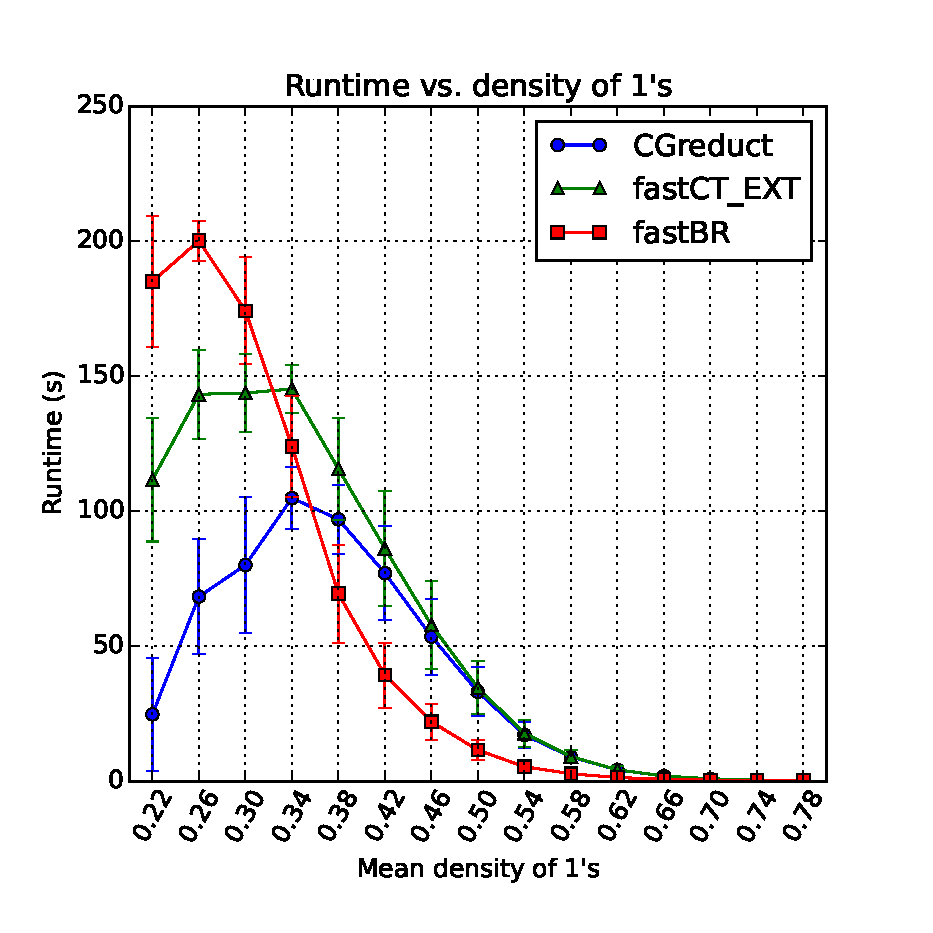
\includegraphics[height=8cm]{imgs/overal.eps}
		\end{center}
		\caption{Average algorithms' runtime vs. density of 1's for all synthetic \textit{SBDMs}.}
		\label{fig:scattDensity}
	\end{figure}	

	For clarity purposes, the 500 synthetic \textit{SBDMs} were divided into 15 bins by discretizing the range of densities, each bin having approximately 33 \textit{SBDMs}. Figure~\ref{fig:scattDensity} shows the average runtime for all  matrices in each bin for the three algorithms, as a function of the density of 1's in the synthetic \textit{SBDMs}. In this figure, the vertical bars show the standard deviation in each bin. 
		
	From Figure~\ref{fig:scattDensity}, we can see that for matrices with density under 0.36  the fastest algorithm was GCreduct, fast--BR was the fastest for matrices with density between 0.36 and 0.66, and the three algorithms show a similar performance for matrices with density above 0.66. The fact that \textit{SBDMs} with a high density do not constitute a complex computational task for reduct computation \citep{Rojas12}, is clearly visible in Figure~\ref{fig:scattDensity}. For this reason, a detailed analysis in this region lacks of relevance.
		
	In order to explain the line delimiting those \textit{SBDMs} for which GCreduct is faster than fast--BR (densities under 0.36), we must go deeply into the main difference between these algorithms. The evaluation of the attribute exclusion is the part with the highest complexity within these algorithms ($\Theta (nm)$). This operation is executed more often in fast--BR than in GCreduct. The attribute exclusion occurs when there is at least one column in the sub-matrix of the \textit{SBDM}, considering only the attributes in the current candidate that can be removed without increasing the number of zero rows in this sub-matrix. The exclusion is more frequent in matrices with a higher density, where overlapping of 1's is more likely. The higher cost of candidate evaluation in fast--BR pays off for \textit{SBDMs} with higher densities (the limit identified from our experiment is 0.36), because supersets of candidates with attribute exclusion are excluded from subsequent evaluations. For instance, taking the extreme case of the identity matrix, where there is no exclusion at all since every attribute is indispensable to form a reduct. For this kind of \textit{SBDMs}, GCreduct needs to evaluate as many candidates as fast--BR but the former makes a single verification for exclusion with the set of all attributes. On the other hand, fast--BR verifies the exclusion for each candidate, which leads to a higher runtime.
	
	The Friedman and post hoc Nemenyi-Damico-Wolfe-Dunn tests show that GCreduct was significantly faster (\textit{p--value} $< 10^{-16}$) than fast--CT\_EXT for low (under 0.36) and medium (between 0.36 and 0.66) density matrices. In relation to fast--BR, GCreduct showed a significant runtime reduction (\textit{p--value} $< 10^{-16}$) for low density matrices while it was significantly slower (\textit{p--value} $< 10^{-16}$) for medium density matrices. From this analysis, we conclude that GCreduct is the best algorithm for low density matrices; while fast--BR is the best for medium density matrices. For high density matrices (over 0.66), any algorithm can be used since, as we already stated, computing reducts on this kind of matrices does not constitute a complex computational task. Moreover, from these conclusions a great advantage can be taken of selecting the appropriate algorithm for a specific decision system, since the density of 1's can be computed a priori with a relatively low computational cost.
	
	\begin{table}[H]
		\centering \footnotesize
		\caption{Fast--CT\_EXT, GCreduct and Fast--BR runtime for decision systems taken from UCI. Sorted by \textit{SBDM} density.}
		\label{tab:density}
		\begin{tabular}{lcrrr}
			\hline
			\multicolumn{1}{c}{Decision}  && Fast--CT\_EXT & \multicolumn{1}{c}{Gcreduct} & \multicolumn{1}{c}{Fast--BR}  \\
			\multicolumn{1}{c}{system}       & Density & runtime (s) & runtime (s)  & runtime (s)  \\
			\hline
			Chess (kr-vs-kp)          & 0.03    & 7.45          & \textbf{$<$0.01} & 0.02            \\
			Keyword-activity          & 0.04    & 1.22          & \textbf{0.42}    & 0.90            \\
			Connect-4                 & 0.05    & 12876.67      & \textbf{44.23}   & 160.61          \\
			QSAR-biodeg               & 0.12    & 0.75          & \textbf{0.19}    & 0.33            \\
			Landsat (train)           & 0.33    & 23797.99      & \textbf{9949.31} & 17732.49        \\
			Dermatology               & 0.34    & 16.02         & 12.25            & \textbf{4.62}   \\
			Credit-g                  & 0.35    & \textbf{0.05} & 0.06             & 0.12            \\
			Flags                     & 0.35    & 1.00          & \textbf{0.74}    & 1.06            \\
			Diabetes                  & 0.38    & 86.99         & \textbf{19.48}   & 23.37           \\
			Student-por               & 0.41    & 1874.57       & 1657.90          & \textbf{161.35} \\
			Sponge                    & 0.42    & 0.63          & 0.58             & \textbf{0.14}   \\
			Student-mat               & 0.43    & 1003.87       & 929.46           & \textbf{81.82}  \\
			Lung-cancer               & 0.47    & 188.20        & 133.43           & \textbf{7.34}   \\
			Waveform                  & 0.50    & 2.11          & 1.88             & \textbf{1.64}   \\
			Cylinder-bands            & 0.55    & 5.03          & 4.59             & \textbf{0.53}   \\
			\hline
		\end{tabular}
	\end{table}

	In Table~\ref{tab:density}, we included the density of 1's and the runtime shown for each \textit{SBDM} in Table~\ref{tab:java}. We also sorted the decision systems of Table~\ref{tab:density} in ascending order of the density of 1's in their associated \textit{SBDM}. Although this is a small heterogeneous sample, the rule obtained from synthetic data can be verified in this table. For decision systems with \textit{SBDM} densities close to the boundary of 0.36 we cannot conclude which is the fastest algorithm, as it can be seen in Table~\ref{tab:density}. However, for those decision systems which have a \textit{SBDM} with density clearly under 0.36, GCreduct was the fastest. In the same way, fast-BR performed faster for those decision systems having a \textit{SBDM} with density clearly above 0.36.
	
	The density of 1's of the \textit{SBDM} is not the only parameter affecting the relative performance of these algorithms. This fact can be verified in Figure~\ref{fig:scattDensity}, where the vertical bars show the standard deviation of the runtime for different \textit{SBDMs} which have the same density. Thus, we may infer that the distribution of 1's within the \textit{SBDM} also has a significant influence, which deserves a deeper study. However, in our experiments, for density values not too close to 0.36 these variations in the distribution of 1's within the \textit{SBDMs} had no effect on the determination of the fastest algorithm, as it can be also seen in Figure~\ref{fig:scattDensity}.
%	
\section{Conclusions}\label{GC_conclusions}
%
	In this chapter, we presented a new algorithm, GCreduct, for computing all reducts of a decision system. In the proposed algorithm, the search space is traversed evaluating some candidate subsets and, based on pruning properties, many others are discarded. Algorithms reported in the literature use operations with a high cost for candidate evaluation, in order to reduce the number of evaluated candidates. The main contribution of our proposal, unlike previous algorithms, is the use of simpler operations for candidate evaluation, based on the pruning properties of gap elimination and attribute contribution, for a faster reduct computation. 
	
	After conducting a series of experiments over synthetic \textit{SBDMs} and decision systems from the UCI repository, we can conclude that GCreduct performs faster than fast--BR and fast--CT\_EXT on those decision systems whose associated \textit{SBDM} has a density of 1's under 0.36. This result provides an instrument to select the proper algorithm for a determined decision system. Further studies should be undertaken to deeply explore the relation found between the fastest algorithm for reduct computation of a decision system and the density of 1's of the associated \textit{SBDM}. 
	
	Finally, since the density of 1's of the \textit{SBDM} is not the only factor affecting the performance of the algorithms for computing reducts, other factors deserve a wider study as future work.


			
\newpage 
%
\chapter[Hardware Implementation]{A New Fast Hardware Software Platform for Computing Reducts} \label{chap:FPGA} 
%TODO modificar todas las imágenes para q digan reduct
%TODO cambiar todo el vocabulario a reductos
%

%
\section{Introduction}
%
	In spite of advances in the theoretical aspects of computing irreducible testors, there are no hardware implementations reported aside from \citep{Cumplido06,Rojas07,Rojas12}. In the first work, an FPGA-based brute force approach for computing testors was proposed~\citep{Cumplido06}. This first approach did not take advantage of dataset characteristics to reduce the number of candidates to be tested; thus all $2^n$ combinations of $n$ attributes have to be tested. Then, in \citep{Rojas07} a hardware architecture of the BT algorithm~\citep{Ruiz85} for computing irreducible testors was implemented. This algorithm uses a candidate pruning process for avoiding many unnecessary candidate evaluation, reducing the number of verifications of the irreducible testor condition. These two previous works computed a set of testors on the FPGA device whilst irreducible condition was evaluated afterwards by the software component in the hosting PC. Thus \cite{Rojas12} proposed a hardware software platform for computing irreducible testors that implemented the BT algorithm, as in \citep{Rojas07}, but it also included a new module that eliminates most of the non irreducible testors before transferring them to a host software application for final filtering. One disadvantage of these approaches is the huge amount of data that must be transferred to the PC. Consequently, in~\citep{Rodriguez14} we proposed a modification to this platform in order to compute irreducible testors in the hardware component. 
	
	Several hardware accelerations have been recently reported for feature selection in Rough Set Theory. Authors of~\citep{Grzes13,Kopczynski14} presented an FPGA based platform for computing a reduct. \cite{Tiwari13} presented various algorithms for attribute reduction using concepts of Rough Set Theory and implemented the Quick Reduct	algorithm in a hardware fashion. Then, \cite{Tiwari14} presented a thorough survey on hardware implementation of rough set algorithms. These hardware implementations aim to compute a single reduct. \cite{Jensen14} addressed the lack of guarantees for finding an attribute subset with minimal cardinality, which is the main drawback of these approaches. 
	
	In this chapter, we present an efficient hardware software platform for computing irreducible testors based on the CT-EXT algorithm~\citep{Sanchez07}. The main contribution of this work is the design and implementation of a hardware architecture that traverses the search space in a different order than that presented in \citep{Rojas07, Rojas12,Rodriguez14}. This new strategy evaluates less candidate subsets than previous architectures, which results in shorter runtime. In comparison to the software versions of CT-EXT~\citep{Sanchez07, Sanchez10}, our proposal evaluates a candidate every clock cycle, which leads to a faster execution. The runtime gain of our new hardware software platform is demonstrated throughout experiments over synthetic datasets. 
	
	The rest of this chapter is structured as follows. Section~\ref{sec:platform} describes the proposed architecture. Evaluation of the proposed platform and a discussion of the experimental results are presented in Section~\ref{sec:evaluationHardware}. Finally, Section~\ref{sec:conlusionsHardware} shows our conclusions and some directions for future work.

%
\section{Proposed platform}\label{sec:platform}
%
	Since the problem of computing all reducts has exponential complexity regarding the number of attributes; our proposed 	platform, as well as any other existing algorithm, has exponential complexity. A common stage to all algorithms for computing irreducible testors is the verification of each candidate combination over the basic matrix. This is an intrinsic parallel operation that a hardware implementation could take advantage of. The time complexity of evaluating a candidate for the testor condition is $O(nm)$ and for the irreducible condition is $O(n^2m)$; where $n$ is the number of attributes and $m$ is the number of rows in the basic matrix. In the proposed hardware component, these conditions are simultaneously evaluated in a single clock cycle. Moreover, the main novelty in this work relays on the Candidate Generator module. This new module implements the lexicographical total order~\citep{Sanchez07} as in the CT-EXT algorithm. This traversing order allows our proposal to evaluate less candidates than those evaluated by other hardware architectures reported in the literature; reducing, in this way, the execution time.
	
	The proposed platform is shown in Figure~\ref{fig:general}. The platform comprises a host PC and an Atlys board populated with a FPGA Spartan-6 device \citep{Digilent2013}; which are connected through a USB cable. A custom developed software application, running in the PC, handles all the processes needed to create the bitstream file to configure the FPGA device. The custom architecture implemented in the FPGA carries out all the calculations needed to generate the testors and sends the results to the PC where the users can then analize the results. A detailed description of all the platform components are given below.
	
	\begin{figure}[htb]
	    \begin{center}
	       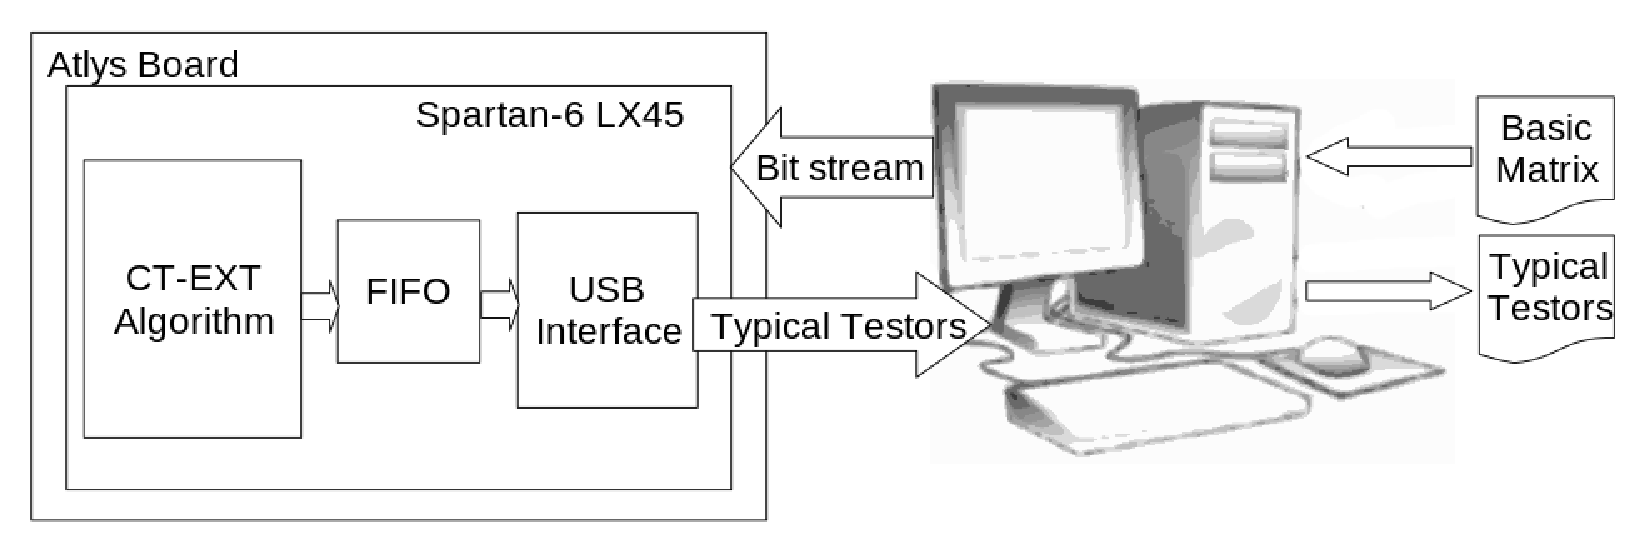
\includegraphics[width=13cm]{imgs/Arquitecture.eps}
	    \end{center}
	\caption{Proposed hardware software platform.}
	\label{fig:general}
	\end{figure}
%	
\subsection{Hardware architecture}\label{sec:architecture}	
%

	In the hardware architecture, an attribute subset is handled as an $n$-tuple, using a positional representation for all the $n$ attributes of a basic matrix $BM$. Given a subset $T$, its $n$-tuple representation has a 1 in the corresponding position $j$ for each $x_j \in T$ and 0 otherwise. The process of deciding whether an $n$-tuple is a testor of $BM$ involves comparing the candidate against each one of the $BM$'s rows. For software-only implementations, this is a big disadvantage, specially for large matrices with many rows. The proposed hardware architecture exploits the parallelism inherent in the CT-EXT algorithm and evaluates whether a candidate is an irreducible testor, or not, in a single clock cycle. The hardware implementation of CT-EXT is composed of two modules, the $BM$ module and the Candidate Generator module, as shown in Figure~\ref{fig:arquitecture}.
		
	\begin{figure}[htb]
	  \begin{center}
	      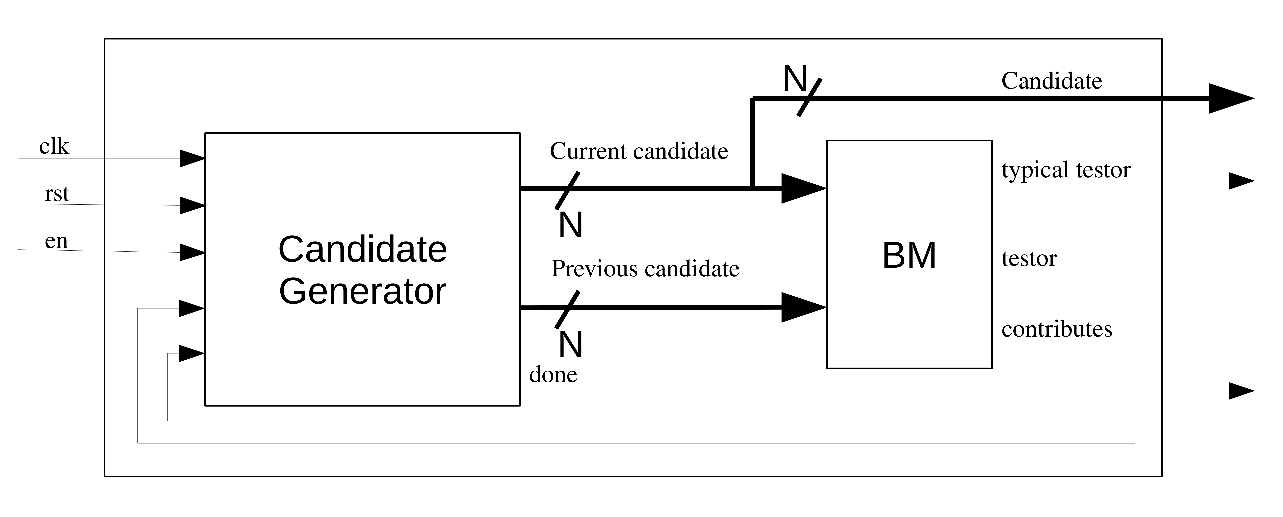
\includegraphics[width=13cm]{imgs/CT-ext_arq.eps}
	  \end{center}
	\caption{CT-EXT Architecture.}
	\label{fig:arquitecture}
	\end{figure}
	
	The $BM$ module stores the input matrix and includes all the logic needed to decide whether an $n$-tuple is a testor. The candidate generator module produces the candidates ($n$-tuples) to be evaluated by the $BM$ module. In order to calculate the next candidate according to the CT-EXT algorithm, the architecture feedbacks the evaluation result of the previous candidate to the generator module; this drastically reduces the number of candidates tested and consequently the number of iterations needed by the algorithm. 	
	
	\begin{figure}[htb]
	    \begin{center}
	        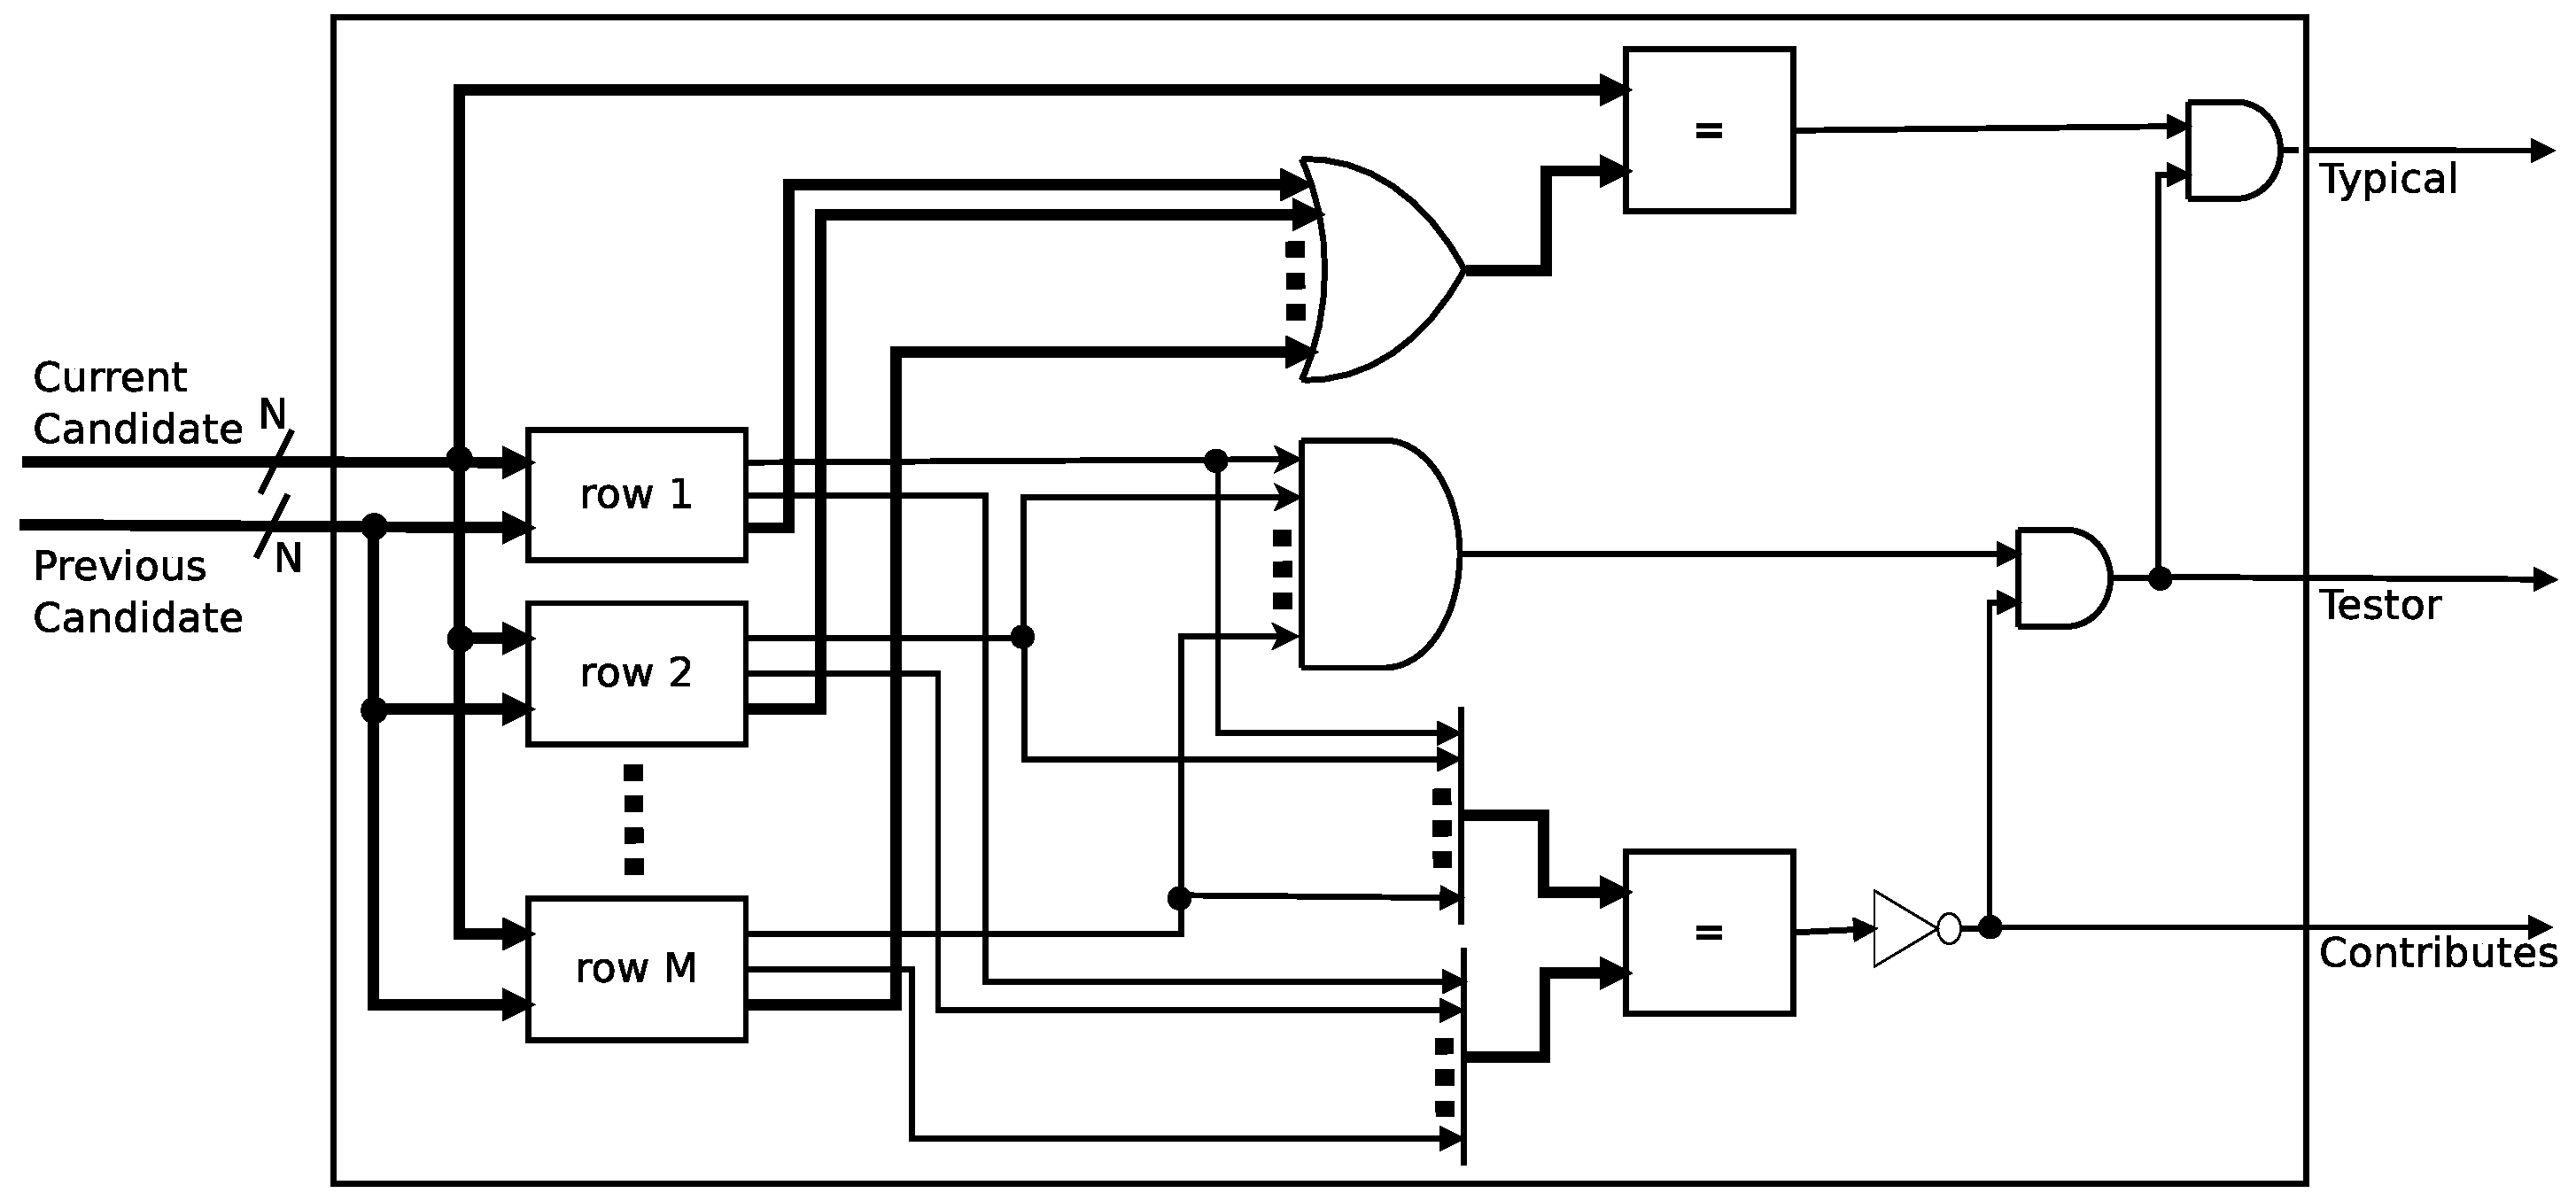
\includegraphics[height=6cm]{imgs/BM_module.eps}
	    \end{center}
	\caption{$BM$ module.}
	\label{fig:bmModule}
	\end{figure}
	
	The $BM$ module is composed of $M$ sub-modules named \textit{row~i}, as shown in Fig.\,\ref{fig:bmModule}. Each \textit{row~i} module contains a row ($n$ bits) of the $BM$ matrix and the logic needed to perform a testor evaluation. To decide whether an $n$-tuple is a testor, a bitwise AND operation is performed between the value stored in each \textit{row~i} module and the current candidate, as shown in Figure~\ref{fig:row}. If at least one bit of the AND operation is TRUE, then the output \textit{Testor} of that particular \textit{row~i} sub-module will be TRUE. The same operation is performed over the previous candidate. If the output \textit{Testor} is different from the output \textit{Contributes} for any \textit{row~i} sub-module, it means that the current candidate reduces the amount of zero rows regarding the previous candidate and then, the output \textit{Contributes} from the $BM$ module becomes TRUE. If the output $Testor$ of all  \textit{row~i} sub-modules is TRUE, then the output \textit{Testor} of the $BM$ module will be TRUE, which means that the candidate is a testor of $BM$.
	
	\begin{figure}[htb]
	    \begin{center}
	        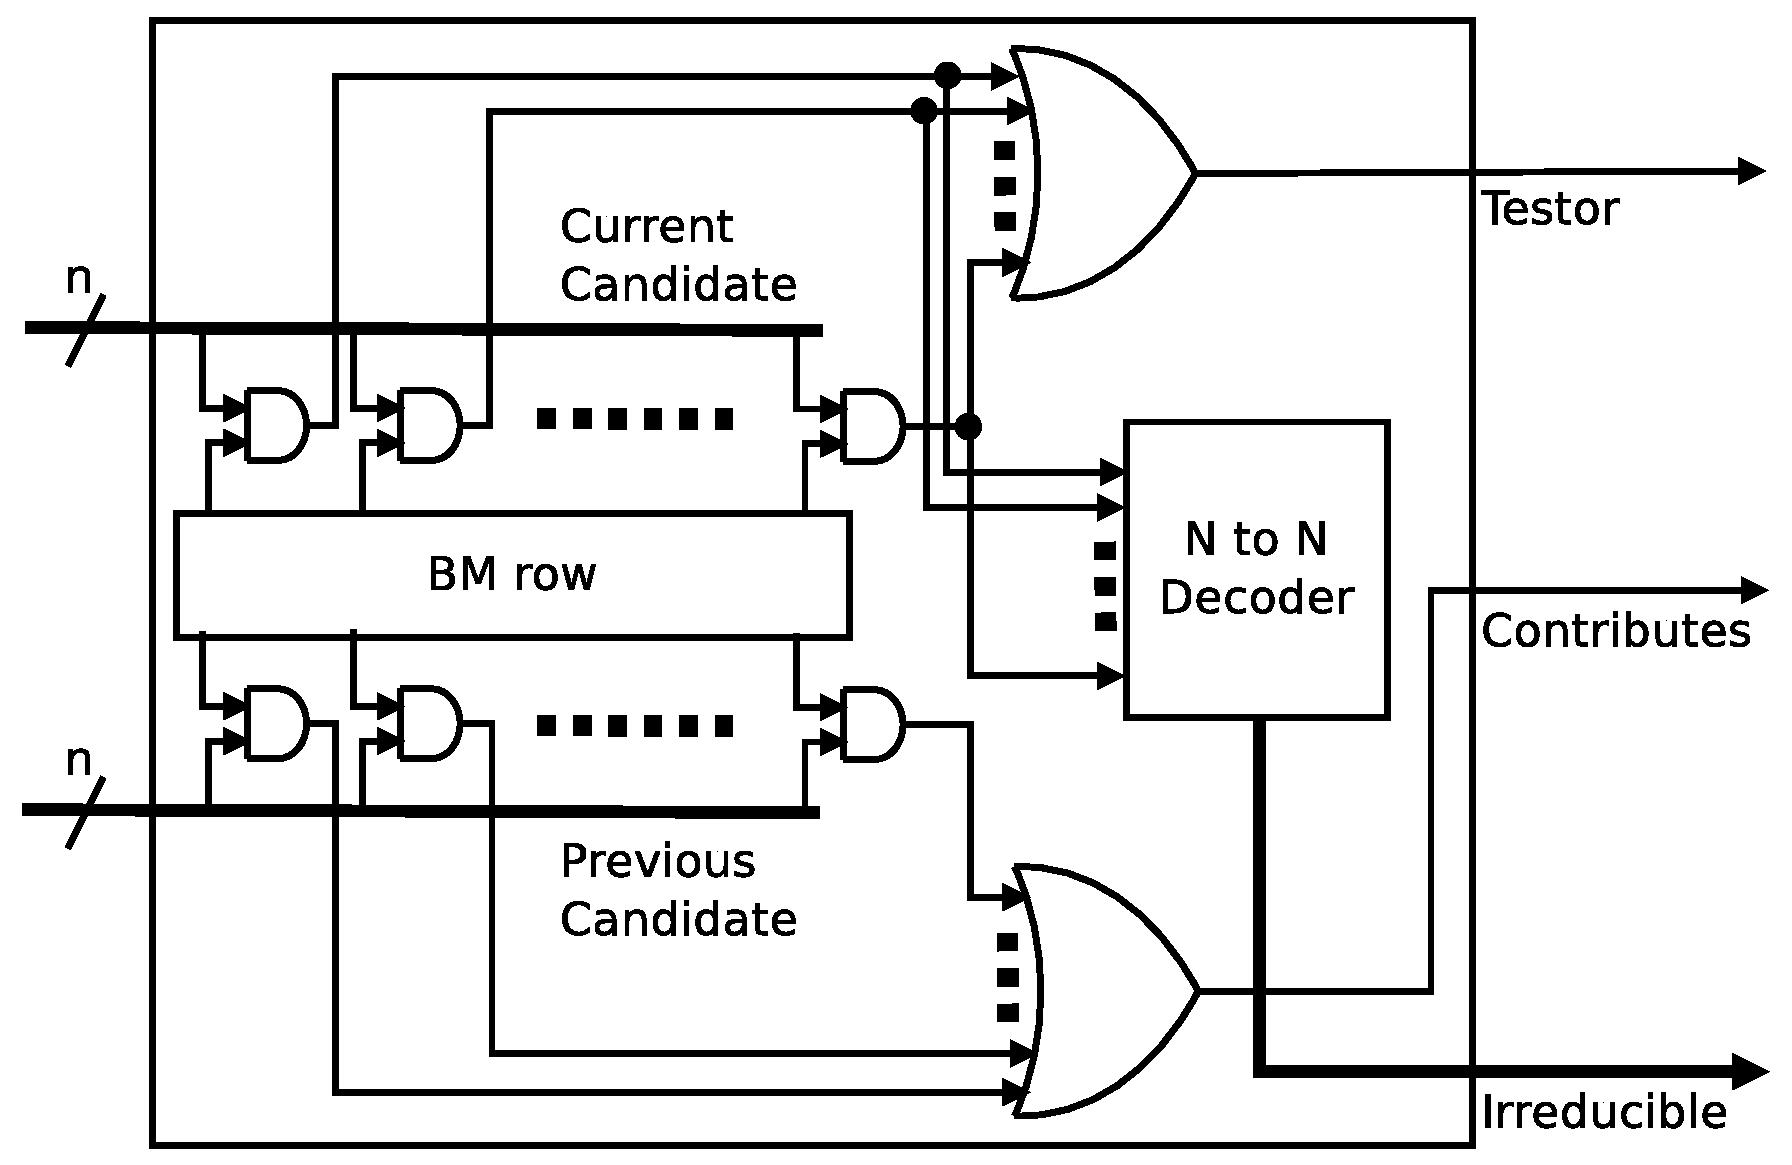
\includegraphics[height=6cm]{imgs/BM_row.eps}
	    \end{center}
	\caption{$BM$ row.}
	\label{fig:row}
	\end{figure}
		
	In order to verify the irreducible condition, an \textit{N~to~N~Decoder} receives as input the result of the AND operation between the current candidate and the corresponding $BM$ row. The output from the \textit{N~to~N~Decoder} repeats the input when there is only one bit set to 1, and returns zero otherwise. For those rows with only one bit having a 1 after ANDed with the candidate, the attribute in the position of that bit is indispensable if the candidate is a testor. According to definition of irreducible testor, every attribute must be indispensable.
	
	\setlength{\tabcolsep}{3pt} %TODO este ejemplo hay q unificarlo
	\begin{table}[!htb]
	    \begin{minipage}{.5\linewidth}
	      \caption{Irreducible testor.}\label{tab:exampleReduct}
	      \centering
	        \begin{tabular}{ ccccc|ccccc }
	 			\hline                       
	  			\multicolumn{5}{c|}{Cand. $\{c_0, c_1\}$} & 
	  			\multicolumn{5}{c}{Decoder output} \\
	  			\hline
				  $c_0$ &   $c_3$ &   $c_4$ &   $c_1$ &   $c_2$ &
	  			  $c_0$ &   $c_3$ &   $c_4$ &   $c_1$ &   $c_2$ \\
	  			\hline
	  			1 & 0 & 0 & 0 & 0 & 1 & 0 & 0 & 0 & 0\\
	  			0 & 0 & 0 & 1 & 0 & 0 & 0 & 0 & 1 & 0\\
	  			1 & 0 & 0 & 1 & 0 & 0 & 0 & 0 & 0 & 0\\
	  			\hline  
	  			\multicolumn{5}{c|}{Candidate $=$} & 1 & 0 & 0 & 1 & 0\\
	  			\hline  
			\end{tabular}
			
	    \end{minipage}%
	    \begin{minipage}{.5\linewidth}
	      \centering
	        \caption{Not irreducible testor.}\label{tab:exampleNonReduct}
	        \begin{tabular}{ ccccc|ccccc }
	 			\hline                       
	  			\multicolumn{5}{c|}{Cand. $\{c_0, c_4\}$} & 
	  			\multicolumn{5}{c}{Decoder output} \\
	  			\hline
	  			  $c_0$ &   $c_3$ &   $c_4$ &   $c_1$ &   $c_2$ &
	  			  $c_0$ &   $c_3$ &   $c_4$ &   $c_1$ &   $c_2$ \\
	  			\hline
	  			1 & 0 & 1 & 0 & 0 & 0 & 0 & 0 & 0 & 0\\
	  			0 & 0 & 1 & 0 & 0 & 0 & 0 & 1 & 0 & 0\\
	  			1 & 0 & 1 & 0 & 0 & 0 & 0 & 0 & 0 & 0\\
	  			\hline  
	  			\multicolumn{5}{c|}{Candidate $\neq$} & 0 & 0 & 1 & 0 & 0\\
	  			\hline  
			\end{tabular}
	    \end{minipage} 
	\end{table}
	%TODO este párrafo hay q unificarlo con la MB de basic concepts
	Taking as example the ordered basic matrix of Table~\ref{tab:SBDM1}. In Table~\ref{tab:exampleReduct} the irreducibility of $\{c_0,c_1\}$ is evaluated while the same is done for $\{c_0,c_4\}$ in Table~\ref{tab:exampleNonReduct}. Left rows show the result of the AND operation between each row of $BM$ and the candidate, while those rows in the right show the decoder output taking as input its corresponding left row. In the last row, the result of an OR operation over all above bits is shown. According to our previous explanation, the candidate $\{c_0,c_1\}$ is an irreducible testor given that the result of the OR operation is equal to the candidate itself; while candidate $\{c_0,c_4\}$ is not. This can be corroborated in Table~\ref{tab:example}.	
	
	\begin{figure}[htb]
	    \begin{center}
	        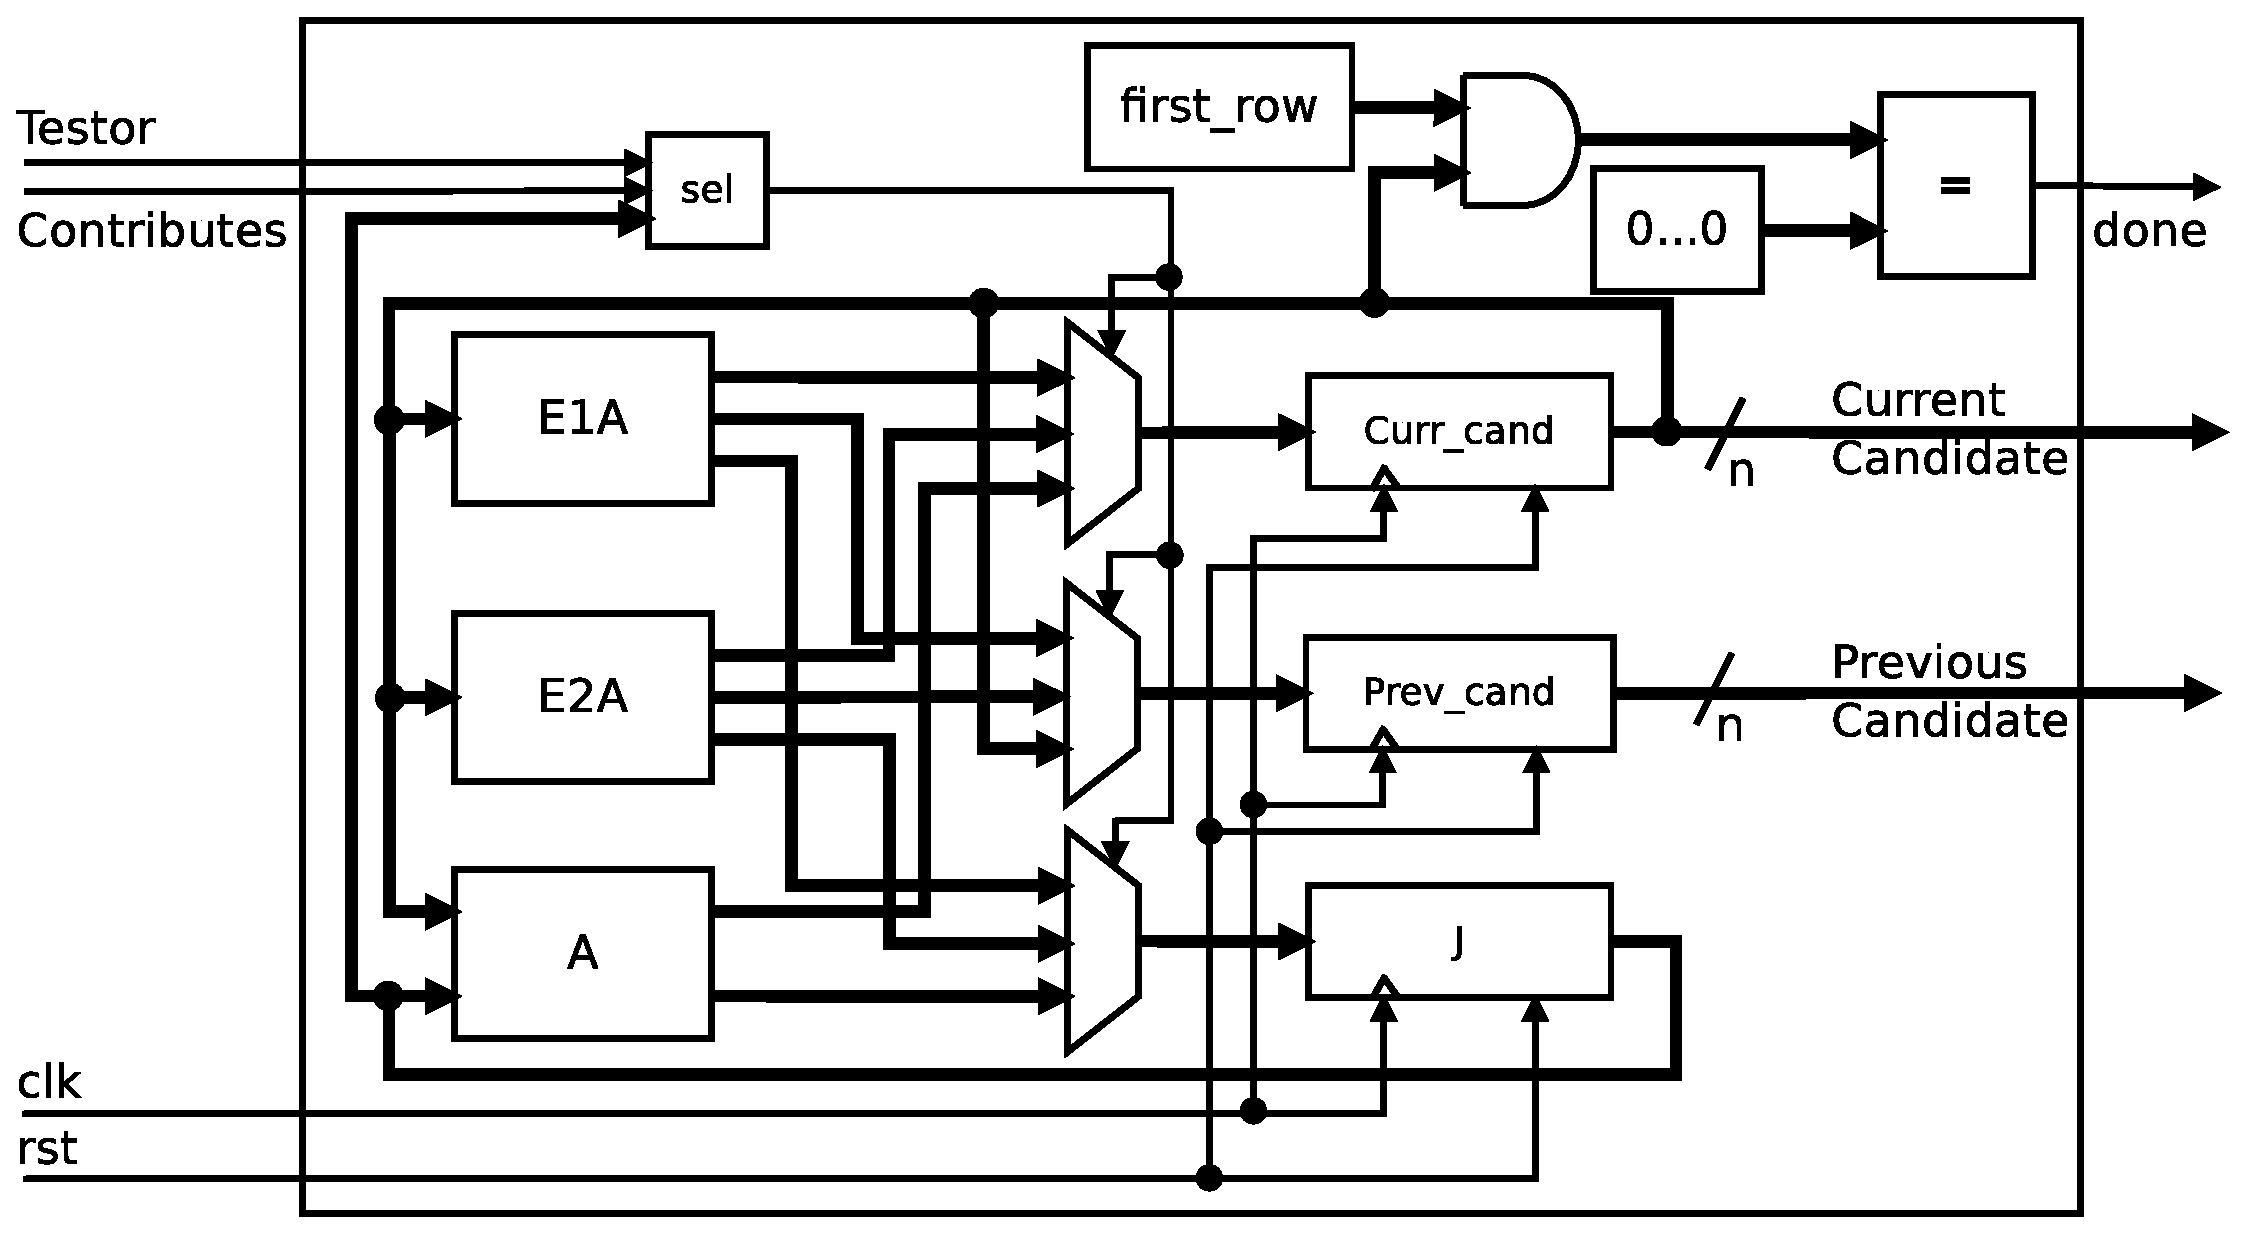
\includegraphics[height=6cm]{imgs/CandGen.eps}
	    \end{center}
	\caption{Candidate Generator module.}
	\label{fig:CG_module}
	\end{figure}
	
	The candidate generator module (Figure~\ref{fig:CG_module}) uses the feedback from the $BM$ module to calculate the next candidate to be evaluated. The candidate generator module consists of three registers for holding the current candidate (\textit{$Curr\_cand$}), the previous candidate (\textit{$Prev\_cand$}) and the last added attribute ($J$). These registers values are updated by the modules EA1, EA2 and A.
	
	Depending on the combination of the input values, the outputs E1A, E2A or A are used for updating the records. Table~\ref{tab_CandGen} shows how the records are updated according to the values of \textit{Testor}, \textit{Contributes} and $J$ inputs. This operation is computed by the module \textit{sel} shown in Figure~\ref{fig:CG_module}.
	
	\begin{table}[htb]
			\caption{Candidate Generator Selector.} \label{tab_CandGen}
			\centering
	 	\begin{tabular}{ccc}
	 			\hline
	 			Priority & Condition & Registers update\\
	 			\hline
	 			1 & \multicolumn{1}{>{\centering\arraybackslash}m{1in}}{$J=J_{max}$
	 				($J_{max}=$ max value of $J$)} & \multicolumn{1}{>{\centering\arraybackslash}m{2in}}{
	 				$Curr\_cand$ $\leftarrow$ E2A
	 				$Prev\_cand$~$\leftarrow$~E2A
	 				$J$~$\leftarrow$~E2A}\\
	 			\hline
	 			2 & \multicolumn{1}{>{\centering\arraybackslash}m{1.2in}}{Contributes $=0$ or Testor $=1$} &
	 			\multicolumn{1}{>{\centering\arraybackslash}m{2in}}{
	 				$Curr\_cand$ $\leftarrow$ E1A
	 				$Prev\_cand$~$\leftarrow$~E1A
	 				$J$~$\leftarrow$~E1A}\\
	 			\hline
	 			3 & \multicolumn{1}{>{\centering\arraybackslash}m{1.2in}}{Contributes $=1$ or Testor $=0$}&
	 			\multicolumn{1}{>{\centering\arraybackslash}m{2in}}{
	 				$Curr\_cand$ $\leftarrow$ A
	 				$Prev\_cand$~$\leftarrow$~$Curr\_cand$
	 				$J$~$\leftarrow$~A}\\
	 			\hline       
	 	\end{tabular}             
	\end{table}
	
	The submodule $A$, shown in Figure~\ref{fig:subA}, assigns 1 to the next attribute at the right of the last bit with value 1 in the input candidate. The outputs of the submodule $A$ are the new candidate and $J+1$.
	
	The submodule $E1A$, shown in Figure~\ref{fig:subEA1}, comprises the \textit{Rem$\_1$} (Figure~\ref{fig:subRem1}) and $A$ submodules. The submodule \textit{Rem$\_1$} deletes the last attribute added to the input candidate. This action is performed by a priority encoder which locates the last bit with value 1 in the input candidate. \textit{Rem$\_1$} outputs represent the previous candidate and the index of the deleted bit. These outputs are connected to the corresponding inputs of the submodule $A$, in order to add an attribute in the corresponding position. Finally, the outputs of $E1A$ represent the new candidate to be evaluated, the previous candidate and the index where the new attribute was added to the current candidate. 
	
	\begin{figure}[htb]
	\centering
	\begin{minipage}{.5\textwidth}
	  \centering
	   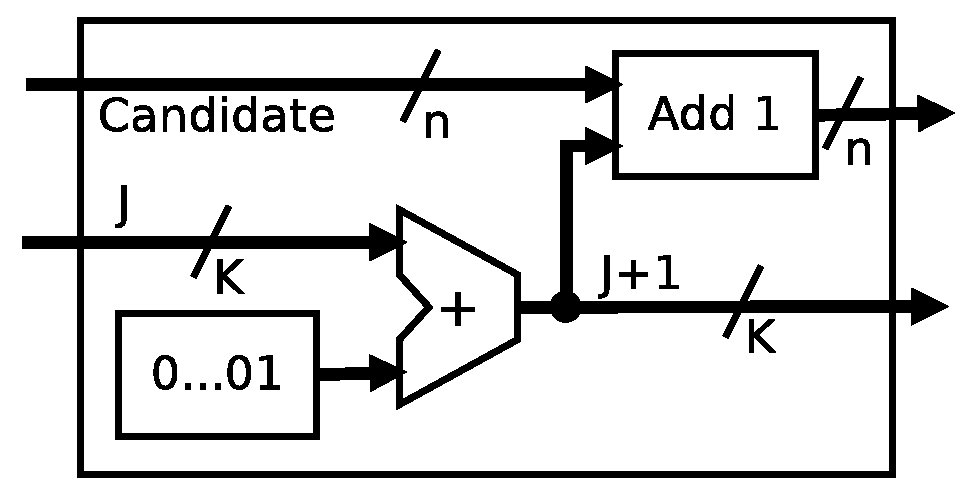
\includegraphics[width=.7\linewidth , height=3cm]{imgs/Add1.eps}
	  \caption{Submodule A.}
	  \label{fig:subA}
	\end{minipage}%
	\begin{minipage}{.5\textwidth}
	  \centering
	   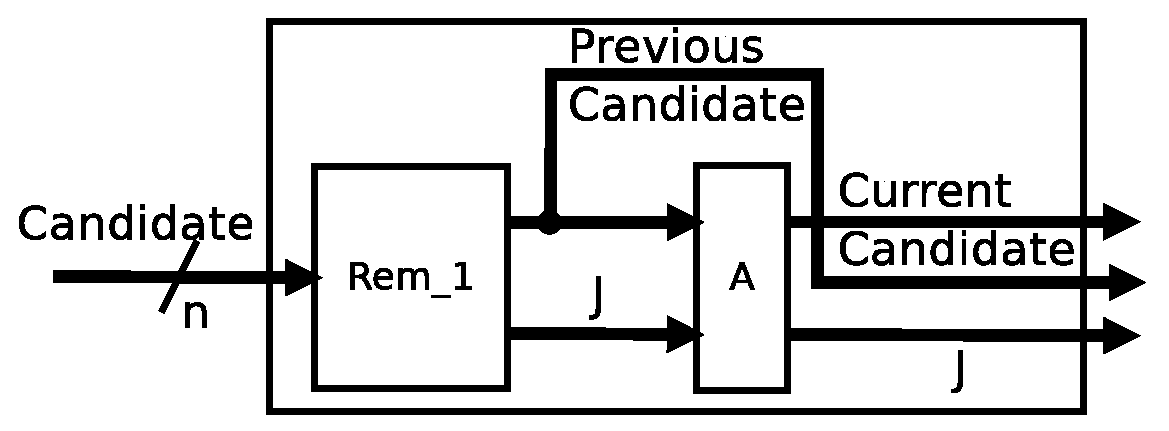
\includegraphics[width=\linewidth , height=3cm]{imgs/EA1.eps}
	  \caption{Submodule E1A.}
	  \label{fig:subEA1}
	\end{minipage}
	\end{figure}
	
	Finally, the submodule $E2A$ removes the last two attributes from the input candidate, and then adds the following corresponding attribute. This operation is performed by means of two \textit{Rem$\_1$} submodules and an $A$ submodule, as shown in Figure~\ref{fig:subEA2}.
	
	In order to check if the execution of the CT-EXT  algorithm has finished, the result of an AND operation between the current candidate and the first row of the basic matrix is compared to the null $n$-tuple ($0,...,0$), as shown in the upper right corner of Figure~\ref{fig:CG_module}. If the result of this comparison is TRUE, then the output $done$ is activated because any further candidate will not satisfy the testor condition over the first row of $BM$. %TODO referenciar esta propiedad
	
	\begin{figure}[htb]
	\centering
	\begin{minipage}{.5\textwidth}
	  \centering
	   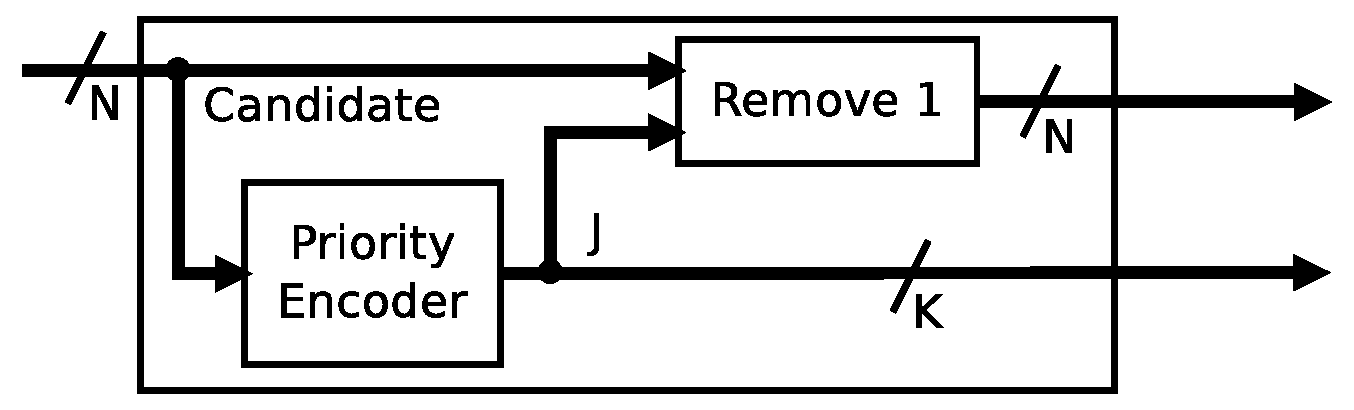
\includegraphics[width=\linewidth , height=3cm]{imgs/Rem1.eps}
	  \caption{Submodule $Rem\_1$.}
	  \label{fig:subRem1}
	\end{minipage}%
	\begin{minipage}{.5\textwidth}
	  \centering
	   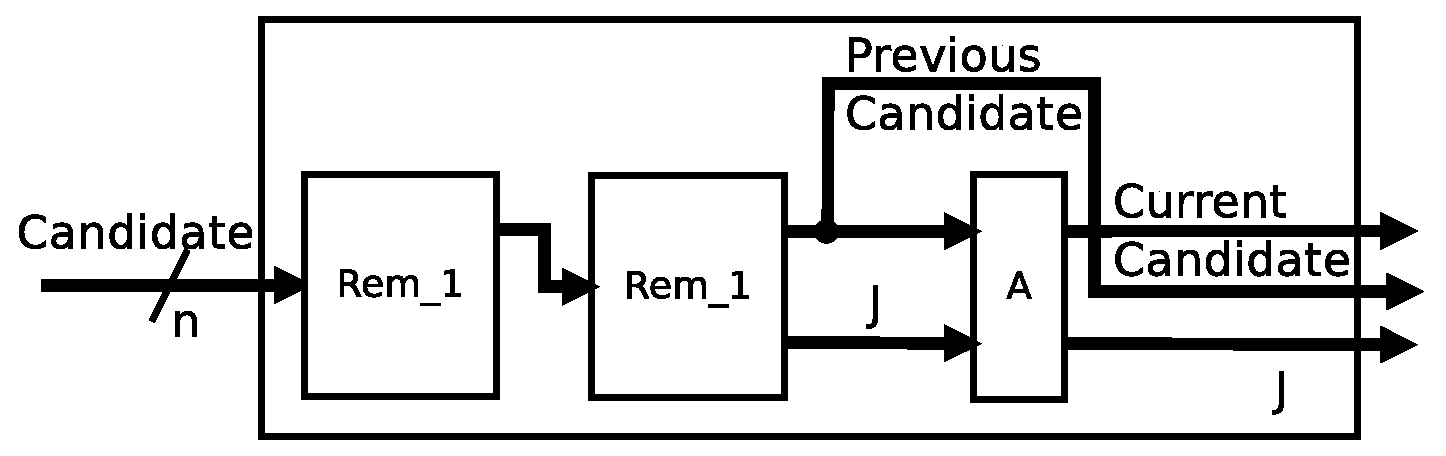
\includegraphics[width=\linewidth , height=3cm]{imgs/EA2.eps}
	  \caption{Submodule E2A.}
	  \label{fig:subEA2}
	\end{minipage}
	\end{figure}

%	
\subsubsection*{The FPGA-based board}
%
	The Atlys board from Digilent \citep{Digilent2013} was selected as the prototyping board. This board is a development and prototyping platform based on a Xilinx Spartan-6 LX45 FPGA, speed grade -3. The Atlys board supports device programming and simplified user-data transfer at a maximum rate of 48MB/s, over a single USB connection. 
	
	The communication between the host PC and the FPGA uses the Digilent Synchronous Parallel Interface (DSTM) protocol~\citep{Digilent2010}. Irreducible testors $n$-tuples, computed by the proposed architecture, are buffered within a FIFO in order to be split into bytes. These bytes are then buffered into a double clocked FIFO~\citep{XilinxInc.2012} to be read from the PC. This last FIFO ensures the output interface operation at 48MHz, as required by the DSTM protocol.

%	
\subsection{Software Description}\label{sect:soft}
%
	The software component allows the user to provide the basic matrix in a plain text file following the format shown in Figure~\ref{fig:8}. The software component is responsible for programming the FPGA device and communicating with the board during irreducible testor computation.

%TODO unificar con el proceso explicado en los otros algoritmos
	First, the basic matrix is reorganized by setting one of the rows with the minimum amount of ones as the first row and swapping columns in such a way those with a 1 in the first row appear on the left. 

	Using the arranged basic matrix, a VHDL file is generated and the synthesis and optimization process is started. This way, the optimization stage takes advantage of the basic matrix data to minimize the FPGA resource utilization. Then, the programming file for the FPGA device is generated.

	On the running stage, the software component interacts with the hardware architecture. First, the device is programmed with the bit-file obtained from the previous stage. Then, the hardware architecture starts computing irreducible testors. The software component keeps pulling through a USB port for new irreducible testors in the output FIFO until the $done$ signal is activated in the FPGA.

%TODO unificar con el proceso explicado en los otros algoritmos
	As a result of the sorting process, the order of attributes in the basic matrix is altered as can be seen comparing Tables~\ref{table1} and~\ref{table2}. Consequently, the irreducible testors calculated in the FPGA must be codified according to the order of columns in the original basic matrix. This task is performed by the software component and then the results are written to the output file.

	\begin{figure}[htb]
	    \begin{center}
	       \includegraphics[height=2.8cm]{imgs/infile.eps}
	    \end{center}
	\caption{Input file format.}
	\label{fig:8}
	\end{figure}
	
\section{Evaluation and Discussion} \label{sec:evaluationHardware}
	In order to show the performance of the proposed platform, it was compared against a software implementation of the CT-EXT algorithm~\citep{Sanchez07} and the BT hardware platform previously reported in~\citep{Rodriguez14}\footnote{The source code of the three implementations and the basic matrix generator, as well as the matrices used for the experiments, can be downloaded from \url{http://ccc.inaoep.mx/~ariel/CTHW/}.}; which is the most recent hardware implementation for computing irreducible testors reported in the literature.
	
	Either CT-EXT or BT hardware implementations are capable of evaluating a candidate per clock cycle. If both architectures are running at the same frequency, as it will be the case in our experiments, there are two reasons for differences in running time. The first one is the time taken for reorganization of basic matrix, which is a more complex process in BT, although it can be neglected as shown in~\citep{Rojas12}. The second and the most relevant, is the amount of candidates to be evaluated. 
	
	Regarding to the software implementation, the CT-EXT hardware platform has two disadvantages. First, VHDL code is generated for each $BM$ data and a process of synthesis must be executed previously to executing the algorithm; while this is unnecessary in the software version of CT-EXT. Secondly, the software will be running in a PC at a frequency of 3.10GHz while FPGA architecture will run at 50MHz. 
	
	These disadvantages make the hardware approach useful (faster) under two conditions. First, the number of candidates to be evaluated is big enough to overcome the synthesis overhead. Second, the dimensions of the $BM$ are big enough to provide a considerable speed up of the candidate evaluation process. Although the hardware architecture could be designed for a fixed maximum matrix size and receive the $BM$ through the USB port, by doing this, the size of the problem which can be solved would be significantly reduced. The synthesis process comprehend an optimization of the design, taking advantage of the $BM$ data distribution for the reduction of the generated hardware configuration. The number of operations for the evaluation of a single candidate, in the software approach, is proportional to the number of rows and it is directly related to the number of columns in the $BM$. Using this approach it is possible to achieve a significant reduction in the processing time, even if operating at a much lower clock frequency, by evaluating a candidate on each clock cycle.
	
	With these points in mind and in order to show the usability of the proposed platform, three kinds of basic matrices were randomly generated. Each type containing different percentage of 1's: 
	\begin{enumerate}
		\item Very-low density matrices: approximately 8\%.
		\item Low density matrices: approximately 33\%.
		\item Medium density matrices: approximately 45\%.
	\end{enumerate}
	
	Higher density matrices were discarded because they do not constitute a computationally expensive problem, as stated by~\cite{Rojas12}. Hereinafter, we will be referring to these three sets of matrices by its approximate density of~1's.
	
	
	\begin{figure}[htb]
	  \centering
	   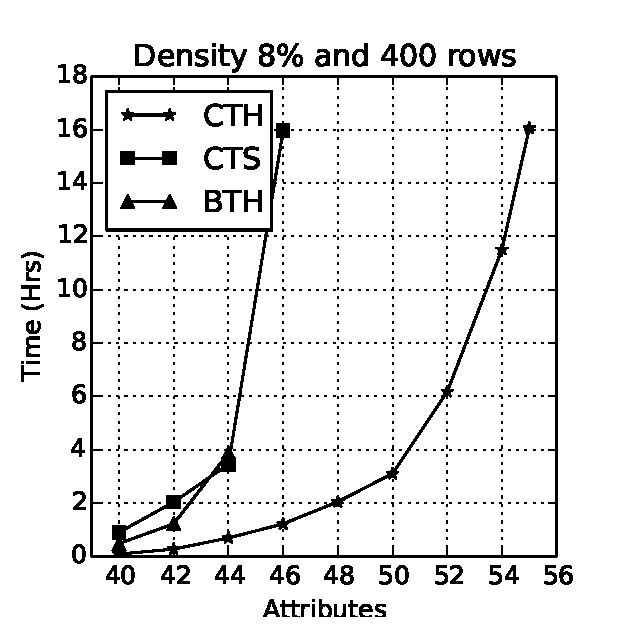
\includegraphics[height=8cm]{imgs/low_density.eps}
	  \caption{Total runtime for density 8\%.}
	  \label{fig:result1}
	\end{figure}
	
	For our experiments, 30 basic matrices of different sizes were randomly generated. A random number generator was used to generate rows, which are filtered for the minimum and maximum number of 1's allowed. In this way the desired density was controlled. If accepted, the row is verified as basic against the saved rows. Basic rows are saved until the desired number of rows is reached. 
	
	\begin{figure}[htb]
	  \centering
	   \includegraphics[height=8cm]{imgs/med_density.eps}
	  \caption{Total runtime for density 33\%.}
	  \label{fig:result2}
	\end{figure}
	
	For the hardware platforms, we measure the runtimes including the time for the following stages: $BM$ input parsing and VHDL code generation, synthesis process, and irreducible testor computation (with the hardware component running at 50MHz). The number of rows for each type of matrices is conditioned by the dimensions of the biggest matrix that may be synthesized at the desired running frequency. All experiments are performed using an Intel(R) Core(TM) i5-2400 CPU @ 3.10GHz for software executions and 
	an Atlys board, powered by a Spartan-6 LX45 FPGA device, for the hardware components. Figures~\ref{fig:result1},~\ref{fig:result2} and~\ref{fig:result3} show graphics of the runtime (in hours) for the three types of basic matrices. 
	
	\begin{figure}[htb]
	    \begin{center}
	       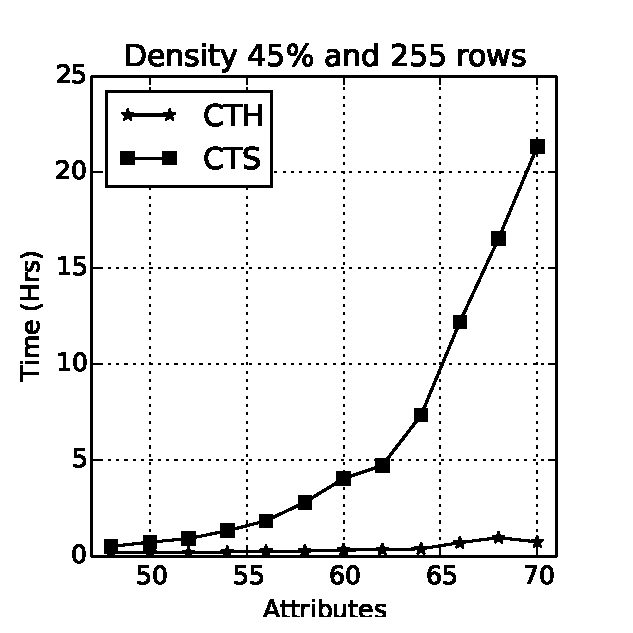
\includegraphics[height=8cm]{imgs/med48_density.eps}
	    \end{center}
	\caption{Total runtime for density 45\%.}
	\label{fig:result3}
	\end{figure}
	
	The proposed CT-EXT hardware platform (CTH) results were taken as reference for axis limits in Figures~\ref{fig:result1},~\ref{fig:result2} and~\ref{fig:result3}. Slowest executions of the CT-EXT software implementation (CTS) are not shown in order to keep clarity in the figures. The hardware platform for BT (BTH) was not able to met the constrain of 50MHz clock frequency for some matrices and running it at a lower frequency produces longer execution time; which fall out of the limits of the figures. We were able to run the three platforms for 4 matrices of different types. 
	
	\cite{Rojas12} stated that the time for computing irreducible testors does not only depend on the size and density of the $BM$. This assertion is illustrated by the matrices with 68 and 70 attributes respectively, in Figure~\ref{fig:result3}. Although these two matrices have a similar density, the larger matrix requires	a shorter execution time.
	
	Table~\ref{table:8} shows the runtime for each stage of the data flow, for 400x40, 400x42 and 400x44 very-low density matrices. This table shows that the synthesis time becomes less significant regarding the total time when the problem size increases. From this table, it can also be seen that the main difference between the BT and CT-EXT hardware implementations is the runtime of the irreducible testor computation process. The main reason for this difference is the number of candidates evaluated by each algorithm. This is an explanation about why the BT hardware implementation is slower than the software version of CT-EXT for the largest matrix in Table~\ref{table:8}.
	
	\begin{table}[htb]
	\caption{Processing time in seconds (broken down for each stage) for 400x40, 400x42 and 400x44 very-low density matrices.} \label{table:8}
	\begin{center}
	    \begin{tabular}{lcccccc}   \hline
	    	   Dimensions                & \multicolumn{2}{c}{400x40} & \multicolumn{2}{c}{400x42} 
	    	                             & \multicolumn{2}{c}{400x44} \\ \hline
	    	    	Stage	        			& CTH & BTH	& CTH & BTH & CTH & BTH \\ \hline
	    	    Load and file generation & 0.05& 0.07& 0.05& 0.06& 0.06& 0.06\\
	    	    Synthesis process        & 253 & 656 & 401 & 564 & 452 & 612\\
	    	    Algorithm execution      & 300 & 1071& 970 & 3826& 2031& 13311\\ \hline
	    	    Total time               & 554 & 1727& 1372& 4390& 2484& 13924\\ \hline
	    	    CTS total time               & \multicolumn{2}{c}{3238} & \multicolumn{2}{c}{7320} 
	    	    								& \multicolumn{2}{c}{12420}\\ \hline	    	    
	    \end{tabular}
	\end{center}
	\end{table}
	
	Tables~\ref{table:6} and~\ref{table:7} summarize the FPGA resource utilization on our prototyping board. The maximum operation frequency from Tables~\ref{table:6} and~\ref{table:7} shows that usually the CT-EXT implementation is potentially faster than the modified BT implementation. Resource utilization is directly related to $BM$ dimensions, its density and to a lesser extent to data organization.
	
	\begin{table}[htb]
	\caption{Synthesis summary of resource utilization for $BM$ with 8\% density on an Spartan-6 LX45 FPGA device.} \label{table:6}
	\begin{center}
	    \begin{tabular}{lcccc}   \hline
	    	    Dimensions & \multicolumn{2}{c}{400x40} & \multicolumn{2}{c}{400x44} \\ \hline
	    	    Algorithm & BT & CT-EXT & BT & CT-EXT \\ \hline
	        Slices & 1,398 (20\%) & 983 (14\%) & 1,554 (22\%) & 1,209 (17\%)  \\
	        6-input LUTs & 4,010 (14\%) & 2,806 (10\%)& 4,475 (16\%)  & 3,004 (11\%)\\
	        Flip-Flops & 832 (1\%) & 852 (1\%) & 876 (1\%) & 938 (1\%)\\
	        Max clock freq & 80.44MHz & 179.58MHz & 84.56MHz & 173.24MHz\\ \hline
	    \end{tabular}
	\end{center}
	\end{table}
	
	\begin{table}[htb]
	\caption{Synthesis summary of resource utilization for $BM$ with 33\% density on an Spartan-6 LX45 FPGA device.} \label{table:7}
	\begin{center}
	    \begin{tabular}{lcccc}   \hline
	    	    Dimensions & \multicolumn{2}{c}{225x50} & \multicolumn{2}{c}{225x55} \\ \hline
	    	    Algorithm & BT & CT-EXT & BT & CT-EXT \\ \hline 
	        Slices & 1,381 (20\%) & 1,554 (22\%) & 1,455 (21\%) & 1,562 (22\%) \\
	        6-input LUTs & 3,769 (13\%) & 4,315 (15\%) & 4,135 (15\%) & 5,026 (18\%)\\
	        Flip-Flops & 949 (1\%) & 980 (1\%) & 1,002 (1\%) & 1,039 (1\%)\\
	        Max clock freq & 87.46MHz & 155.40MHz & 85.27MHz & 156.35MHz\\ \hline
	    \end{tabular}
	\end{center}
	\end{table}
	
	As it was shown in the previous section, the proposed hardware platform provides higher processing performance than the software implementation of the CT-EXT algorithm for the matrices used in our experimentation. This behaviour is possible because the hardware component of the proposed platform is capable of testing whether a candidate is a testor of a $BM$ in a single clock cycle, independently of the number of columns and rows, whereas the software implementation runtime will significantly increase for matrices with a large number of rows.
	
	Experiment results show that the proposed platform beats the software implementation of the CT-EXT algorithm, with ratios of around \textbf{one order} of magnitude. However, for large enough datasets this improvement could be significantly higher, as can be inferred from Figure~\ref{fig:result3}.

%	
\section{Conclusions} \label{sec:conlusionsHardware}
%

	In this chapter, we presented the design and implementation of a new hardware software platform for computing all irreducible testors in a dataset.  Unlike most of the existing hardware architectures for feature selection, our proposal computes all the minimal subsets of attributes that preserve the classification accuracy of the original dataset. The good performance of our hardware implementation, compared to the software approach, is feasible due to the high level of parallelism implicit in the candidate evaluation process of the CT-EXT algorithm; which can be efficiently implemented on an FPGA. This proposed architecture offers an alternative to previous hardware implementations; being faster in most of the cases, by evaluating less candidates to be irreducible testors. 
	
	Experiments also showed that the proposed platform uses fewer hardware resources and it is able to run at a higher clock frequency than previous hardware implementations. This characteristic allows processing larger matrices, since the maximum size of the problem that can be solved in a hardware architecture is conditioned by its resource utilization. Our approach enables the application of Testor Theory methods in larger classification and decision-making problems than it was possible before. 
	
	Even though our platform can process larger basic matrices than previous ones, its resource utilization determines the maximum size of the basic matrix that can be solved (this is, indeed, the main limitation of our proposal), for this reason, the search for new algorithms that could be efficiently implemented on an FPGA constitutes the main direction for future work. Improvements, such as testing two or more candidates at the same time, are still unexplored and would be evaluated in further studies.

%	
\chapter{Conclusions} \label{chap:Conclusions}
%

\section{Conclusions} \label{sec:Conclusions}

Regarding our study about the effect of class imbalance on quality measures for patterns, based on our experimental results, we can conclude that:


\section{Future work} \label{sec:Futurework}

\section{Publications} \label{sec:Publications}


\singlespace 

\textbf{JCR Journals:}

%\begin{itemize}
%% JournalDetail function has two parameters, first one is the impact factor of the journal, and the second one is the quartile of the journal. All based on the JCR report.
%%\item my publications. \JournalDetail{4.529}{1}
%\end{itemize}

\singlespace
\small
\addcontentsline{toc}{chapter}{Bibliography}
\bibliographystyle{apalike}
\bibliography{mybib}

\pagestyle{fancy}
\normalsize
\appendix
\addtocontents{toc}{\protect\setcounter{tocdepth}{0}}

\chapter{some appendix} \label{app:StatisticalTests}



%\backmatter

\end{document}
